%!TEX root = Slides.tex
\part{Indizes und Hashverfahren}

\section{Grundlagen Indizes}

\begin{frame}{Motivation}
\framesubtitle{Analogie: Index eines Buches}
\structure{\textbf{Daumenindex}}
\\[4pt]
\begin{columns}
	\begin{column}{.2\textwidth}
		\includegraphics[scale=0.32]{img/index1.png}
	\end{column}
	\begin{column}{.7\textwidth}
		\begin{itemize}
			\item Daumenindex ordnet logisch zusammenh\"angende Inhalte (Datenwerte) den Abschnitten des Buches (Adressen) zu.
			\item Jedem logischen Inhalt wird ein Abschnitt zugewiesen.
			\item Die Inhalte sind im Daumenindex sortiert/geordnet.
		\end{itemize}
	\end{column}
\end{columns}
\end{frame}

\begin{frame}{Motivation}
\framesubtitle{Analogie: Index eines Buches}
\structure{\textbf{Sachindex}}
\\[4pt]
\begin{columns}
\begin{column}{.33\textwidth}
	\includegraphics[scale=0.4]{img/index2.png}
\end{column}
\begin{column}{.67\textwidth}
	\begin{itemize}
		\item Sachindex ordnet Sachbegriffe (Datenwerte) den Seitenzahlen (Adressen) zu. 
		\item Jedem Sachbegriff k\"onnen mehrere Seitenzahlen zugewiesen werden.
		\item Die Sachbegriffe sind im Sachindex sortiert/geordnet.
	\end{itemize}
\end{column}
\end{columns}
\end{frame}

\begin{frame}{\insertsection}
\framesubtitle{\insertsubsection}	
\begin{definition}[Index]
	Ein Index einer Relation ist eine zus\"atzliche Datenstruktur, die einen effizienten Zugriff auf die Datens\"atze der Relation
	erm\"oglicht. 
	\pause
	\begin{itemize}
		\item Ein Index besteht aus bestimmten Index-Feldern und Adressfeldern.
		\item	Die Index-Felder entsprechen Feldern der Relation. 
		\item Die Werte der Index-Felder bestimmen die Adressen der Seiten der Relation, die die Datens\"atze 
		mit den entsprechenden Feldwerten enthalten. 
	\end{itemize}
\end{definition}		
\end{frame}

\begin{frame}{\insertsection}
\framesubtitle{\insertsubsection}
\begin{figure}
	\includegraphics[scale=0.4]{img/IndexSchema.png}
	\\[-10pt]\caption{Indexstruktur und Relationenschema}
\end{figure}
\end{frame}

\begin{frame}{\insertsection}
\framesubtitle{\insertsubsection}
\begin{figure}
\includegraphics[scale=0.4]{img/IndexPageRelation.png}
\\[-10pt]\caption{Index und Seiten der Relation}
\end{figure}
\end{frame}

\begin{frame}{\insertsection}
\framesubtitle{\insertsubsection}	
\begin{block}{\textbf{Bemerkung}}
	\begin{itemize}
		\item Index wird über einem oder mehreren Feldern (Attributen) der Relation gebildet.
		\item Beliebige Attribute können zur Erstellung des Index herangezogen werden.
		\pause
		\item Index ist zus\"atzliche Datenstruktur, die effizienten Zugriffspfad auf Datens\"atze erm\"oglicht.  	
		\item Index ben\"otigt zus\"atzlichen Speicherbedarf und Aufwand bei Indexverwaltung.				
	\end{itemize}
\end{block}
\abs
\begin{block}{\textbf{Bemerkung}}
	\begin{itemize}
		\item Index-Typen: Dense Index und Sparse Index
		\item Index-Arten: Prim\"arindex und Sekund\"arindex
		\item Index-Klassen: 
		\begin{itemize}
			\item Einstufige und mehrstufige Indizes
			\item B\"aume
			\item Hashing
		\end{itemize}
	\end{itemize}
\end{block}
\end{frame}

\begin{frame}[label=sparsedense]{\insertsection}
\framesubtitle{\insertsubsection}
\structure{Index-Typen}
\abs
Ein Index speichert
\begin{itemize}
	\item die Werte der Index-Felder in sortierter/geordneter Reihenfolge.
	\begin{itemize}
		\item Effiziente Sortierverfahren können angewendet werden
		\item Sequentielle Suche entfällt
	\end{itemize}
	\item eine Menge von zugeh\"origen Adressen auf die Seiten (Bl\"ocke), in denen ein Datensatz mit dem entsprechenden Wert 
	der Felder vorhanden ist. 
\end{itemize}
\pause
\structure{Zwei grundlegende Index-Typen:}
\begin{itemize}
	\item \textit{Dense Index}: Ein Eintrag im Index f\"ur jeden Feld-Wert der Relation
	\item \textit{Sparse Index}: Nur einige Datens\"atze der Relation sind im Index repr\"asentiert. Es existieren Werte-L\"ucken. 
	\begin{itemize}
		\item Notwendige Voraussetzung für einen Sparse Index: nach dem Suchfeld sortierte/geordnete und ggf.~verpointerte Datens\"atze in der
		Relation.
	\end{itemize}
\end{itemize}
\end{frame}

\begin{frame}{\insertsection}
\framesubtitle{\insertsubsection}	
\structure{Index-Arten}
\abs
\textbf{Prim\"arindex}
\begin{itemize}
	\item Prim\"arindex legt neben effizientem Zugriff auch physische Sortierung/Anordnung der 
	indizierten Relation fest.\\[4pt]
	\item Prim\"arindex und Relation sind nach den gleichen Feldern sortiert/geordnet.
	\item F\"ur jede Relation gibt es somit nur einen Prim\"arindex.\\[4pt]
	\item In der Regel wird der Prim\"arschl\"ussel der Relation als Index-Feld verwendet.
\end{itemize}
\pause
\abs
\textbf{Beispiel:} In Mitarbeitertabelle kann Mitarbeiter mit Prim\"arindex f\"ur Schl\"ussel
\texttt{MID} schnell gefunden werden, ohne alle Datens\"atze der Relation direkt zu lesen.	
\\[4pt]
\pause
Beachte: Relation und Prim\"arindex werden \"uber \texttt{MID} sortiert/geordnet gespeichert.
\end{frame}

\begin{frame}{\insertsection}
\framesubtitle{\insertsubsection}	
\structure{Index-Arten}
\abs
\textbf{Sekund\"arindizes}
\begin{itemize}
	\item sind Indizes, die neben dem Prim\"arindex definiert werden.\\[4pt] 
	\item erm\"oglichen weitere effiziente Zugriffspfade auf die Datens\"atze.
\end{itemize}
\pause
\ \\[4pt]
Folge:
\begin{itemize}
	\item Sekund\"arindizes bestimmen nicht Reihenfolge/Ordnung der Datens\"atze im Speicher, sondern geben direkt den Speicherort an.
	\item D\"unn besetzte Sekund\"arindizes (sparse) sind somit sinnlos. Sekund\"arindizes sind immer dicht besetzt (dense).
	\item Suche ist i.~d.~R.~teurer, da Datens\"atze nach einem anderen Schl\"ussel sortiert sind $\Rightarrow$ Keine bin\"are Suche m\"oglich.
\end{itemize}
\end{frame}

\begin{frame}{\insertsection}
\framesubtitle{\insertsubsection}	
\structure{Index-Arten}
\abs
\structure{\textbf{Sekund\"arindizes} -- Anwendungsf\"alle}
\begin{itemize}
\item Unterst\"utzung von schnellen Selektionsbedingungen auf Nicht-Prim\"arschl\"ussel-Attributen
\item Datens\"atze liegen nicht sortiert vor: Sekund\"arindex auf Prim\"arschl\"ussel
\end{itemize}
\pause
\abs\ \abs
\textbf{Beispiel:} In Mitarbeitertabelle k\"onnen mit Sekund\"arschl\"ussel für Attribut 
\texttt{Geburtsdatum} Mitarbeiter mit bestimmtem Geburtstag gefunden werden, ohne in den Datens\"atzen die 
Geburtsdaten zu pr\"ufen.
\\[4pt]
Beachte: Sekund\"arindex kann Sortierung/Ordnung nach \texttt{MID} i.~d.~R.~nicht optimal nutzen.
\end{frame}

\begin{frame}{\insertsection}
\framesubtitle{\insertsubsection}	
\structure{Index-Arten}
\abs
Vergleich mit Buchindizes
\begin{itemize}
	\item Prim\"arindex entspricht Daumenindex\\[8pt]
	\item Sekund\"arindex entspricht Sachindex
\end{itemize}
\end{frame}

\section{Einfache Indexstrukturen}

\subsection{Einfacher Prim\"arindex}

\begin{frame}{\insertsection}
	\framesubtitle{\insertsubsection}
	\structure{\textbf{Einfacher Prim\"arindex auf Prim\"arschl\"ussel}}
	\begin{itemize}
		\item Die Relation ist nach ihrem Prim\"arschl\"ussel sequenziell geordnet.
	  \item Index f\"ur den Prim\"arschl\"ussel. Besteht aus Schlüssel-Pointer-Paaren $(K,P)$
	  \begin{itemize}
	  	\item Pointer $P$ zeigt auf Datensatz, der den Prim\"arschlüsselwert $K$ hat.
	  \end{itemize}
    \item Index-Tupel $(K,P)$ sind nach $K$ sequenziell geordnet gespeichert -- ggf.~im fixed-length-Modus.
  \end{itemize}
\pause
\abs
Zwei M\"oglichkeiten:
\begin{itemize}
	\item Ein Eintrag $(K,P)$ im Index für jeden Wert $K$, der in der Relation vorkommt $\Rightarrow$ Dense Index
	\item Nur einige Datens\"atze der Relation im Index repräsentiert, z.~B.~ein Eintrag je Block $\Rightarrow$ Sparse Index	
\end{itemize}
\end{frame}
  
\begin{frame}{\insertsection}
\framesubtitle{\insertsubsection}
\structure{\textbf{Einfacher Prim\"arindex auf Prim\"arschl\"ussel -- Dense Index}}
\\[4pt]
\begin{columns}[T]
	\begin{column}{.33\textwidth}
		\includegraphics[scale=0.25]{img/Index_Primary-Simple-Dense.png}
	\end{column}
	\begin{column}{.67\textwidth}
		\begin{itemize}
			\item Schl\"ussel-Pointer-Paare im Index
			\item Jeder Schl\"ussel der Daten ist durch ein Paar im Index repräsentiert
			\begin{itemize}
				\item Aber: Wesentlich kleinere Datenmenge
				\item Passt womöglich in den Hauptspeicher
				\item Nur ein I/O pro Zugriff
			\end{itemize}
			\item Sortierung der Paare = Sortierung der Daten		  
		\end{itemize}
	\end{column}
\end{columns}
%	\alert{Pro Block der Datendatei existiert ein Eintrag auf den ersten Record des Blocks im Primary Index -- 
%		es handelt sich daher um einen \textit{sparse Index} (vgl. Folie \ref{sparsedense}).}	
\end{frame}

\begin{frame}{\insertsection}
\framesubtitle{\insertsubsection}
\structure{\textbf{Einfacher Prim\"arindex auf Prim\"arschl\"ussel -- Sparse Index}}
\\[4pt]
\begin{columns}[T]
\begin{column}{.33\textwidth}
	\includegraphics[scale=0.23]{img/Index_Primary-Simple-Sparse.png}
\end{column}
\begin{column}{.67\textwidth}
	\begin{itemize}
		\item Nur ein Index-Tupel $(K,P)$ pro Block: minimaler Prim\"arschl\"usselwert $K$, Pointer $P$ auf Block mit Pointer $P$.
		\item Weniger Speicherbedarf
		\item Aber etwas h\"oherer Suchaufwand. \textbf{Warum?}\\[8pt]
		\item Beispiel
		\begin{itemize}
			\item 100.000 Datenblöcke, 100 Indexpaare pro Block $\Rightarrow$ 1.000 Blocks für Index  $\Rightarrow$ 4MB
		\end{itemize}
	\end{itemize}
\end{column}
\end{columns}
\end{frame}

\begin{frame}{\insertsection}
\framesubtitle{\insertsubsection}
\structure{\textbf{Einfacher Prim\"arindex auf Prim\"arschl\"ussel -- Sparse Index}}
	\begin{figure}
	\includegraphics[width=300pt]{img/PrimaryIndex.pdf}
	\caption{Sparse Primary Index mit Zeiger auf Datendatei-Seiten -- sortiert}
	\end{figure}
\end{frame}

\begin{frame}{\insertsection}
\framesubtitle{\insertsubsection}
\structure{\textbf{Einfacher Prim\"arindex auf Prim\"arschl\"ussel -- Sparse Index}}
\abs
\structure{\textbf{Direkte Suche in Datenbl\"ocken (ohne Index)}}
\abs
\structure{Gegeben sei die folgende sortierte Datendatei:}
\begin{itemize}
	\item Relation mit $N= 30.000$ Datens\"atzen
	\item Block-Gr\"o\ss e: $B = 1024$ Bytes
	\item Datensatzl\"ange: $R = 100$ Bytes (Fixed)
	\item Blockorganisation: Unspanned
\end{itemize}
\abs
\pause
Berechne Anzahl Zugriffe bei direkter Suche nach Datensatz ohne Prim\"arindex:
\begin{itemize}
	\item $bfr=\left \lfloor\frac{B}{R}\right\rfloor = \left \lfloor\frac{1.024}{100}\right\rfloor = 10 \Rightarrow$ 
	$\left\lceil\frac{N}{bfr}\right\rceil = \left\lceil\frac{30.000}{10}\right\rceil = 3.000$ Bl\"ocke für Speicherung
	\item Bin\"are Suche auf in den Bl\"ocken: $\log_2 3000 \approx \mathbf{12}$ \textbf{Zugriffe}
\end{itemize}
\end{frame}

\begin{frame}{\insertsection}
\framesubtitle{\insertsubsection}
\structure{\textbf{Einfacher Prim\"arindex auf Prim\"arschl\"ussel -- Sparse Index}}
\abs
\structure{\textbf{Suche mit Index}}
\begin{itemize}
\item Block-Größe: $B=1024$ Bytes
\item Sortierschlüssel-Länge: $9$ Bytes$\quad$/$\quad$Pointer-Länge: $6$ Bytes
\item Somit: L\"ange eines Datensatzes im Prim\"arindex $r=15$ Bytes
\item Jeder der $3000$ Datenbl\"ocke hat eigenen Eintrag im Index $\Rightarrow n=3000$ Datens\"atze im Index
\end{itemize}
\abs
\pause
Berechne Anzahl Zugriffe bei Suche nach Datensatz mit Prim\"arindex:
\begin{itemize}
\item $bfr_I=\left \lfloor\frac{B}{r}\right\rfloor =\left \lfloor\frac{1.024}{15}\right\rfloor = 68, \Rightarrow$ 
$\left\lceil\frac{3000}{68}\right\rceil = 45$ Bl\"ocke für den Index benötigt
\pause
\item Binäre Suche auf der Index-Datei: $\log_2 45 \approx 6$ Zugriffe
\pause
\item Weitere Zugriff, um passenden Datensatz im Block zu suchen $\Rightarrow 7$ Zugriffe. 
Somit Reduktion um 5 Zugriffe: \textbf{Verbesserung um} $\mathbf{42\%}$ 
\end{itemize}
\end{frame}

\begin{frame}{\insertsection}
\framesubtitle{\insertsubsection}
\structure{\textbf{Einfacher Prim\"arindex auf Prim\"arschl\"ussel -- Sparse Index}}
\abs
\structure{\textbf{L\"oschen und Einf\"ugen von Datens\"atzen}}
\begin{itemize}
	\item Datensatz wird in Daten-Seite eingef\"ugt / gel\"oscht
	\begin{itemize}
		\item Position muss bestimmt werden 
		\item E: Ggf.~muss für neuen Datensatz Platz geschaffen werden $\Rightarrow$ neue Seite
		\item L: Ggf.~wird Inhalt der Seite (des Blocks) geleert $\Rightarrow$ Seite entfernen
	\end{itemize}
	\ \\[4pt]
	\item Index:
	\begin{itemize}
		\item Ist der Datensatz der erste (E) / letzte (L) im Block, so muss der Index angepasst werden
		\item Verschieben sich durch Reorganisationen der Datendatei die Seitenadressen, muss der Index erneut angepasst werden.
	\end{itemize}
\end{itemize}
\end{frame}

\begin{frame}{\insertsection}
\framesubtitle{\insertsubsection}
\structure{\textbf{Einfacher Prim\"arindex auf Prim\"arschl\"ussel -- Sparse Index}}
\abs
\structure{\textbf{Zusammenfassung}}
\begin{itemize}
	\item Datendatei und sortierter Prim\"arindex sortiert $\Rightarrow$ binäre Suche m\"oglich\\[6pt]
	\pause
	\item Suche eines Datensatzes über Prim\"arindex ist effizienter als \"uber Datendatei: 
	\begin{itemize}
		\item Datens\"atze im Index sind kleiner
		\item Folge: Blocking Factor erhöht sich $\Rightarrow$ Reduktion der Anzahl Blockzugriffe
		\item Prim\"arindex ist sparse. Nicht für jeden Schl\"usselwert Index-Eintrag
		\item Folge: Datenmenge im Index verringert sich, Anzahl Blockzugriffe nochmals reduziert.
	\end{itemize}
	\ \\[4pt]
	\pause
	\item Änderungen bei Einf\"ugen/L\"oschen m\"ussen sich auch im Index widerspiegeln.
\end{itemize}
\end{frame}

\begin{frame}{\insertsection}
\framesubtitle{\insertsubsection}
\structure{\textbf{Einfacher Prim\"arindex auf Nicht-Schl\"ussel-Feldern}}
\\[4pt]
\begin{itemize}
\item Index-Felder repr\"asentieren Nicht-Schl\"ussel-Felder der Relation 
\item Die Datens\"atze der Relation sind in den Seiten nach diesen Feldern sortiert/geordnet
\item Ggf.~sind die Seiten entsprechend ver-pointert	
\end{itemize}
\abs
Im folgenden einige einfache Formen von Prim\"arindizes auf Nicht-Schl\"ussel-Feldern
\end{frame}

\begin{frame}{\insertsection}
\framesubtitle{\insertsubsection}
\structure{\textbf{Einfacher Prim\"arindex auf Nicht-Schl\"ussel-Feldern -- Dense Index (Variante 1)}}
\\[4pt]
\begin{itemize}
\item Index besteht aus Feldwert-Adress-Paaren $(K,P)$ f\"ur alle Datens\"atze der Relation mit Feld-Werte $K$.
\item Die Adressen $P$ sind die Adressen der Seiten, in denen sich der Datensatz befindet.
\item Mehrere Feldwert-Adress-Paare im Index f\"ur einen Feld-Wert $K$ m\"oglich.
\end{itemize}
\end{frame}

\begin{frame}{\insertsection}
\framesubtitle{\insertsubsection}
\structure{\textbf{Einfacher Prim\"arindex auf Nicht-Schl\"ussel-Feldern -- Dense Index (Variante 2)}}
\\[4pt]
\begin{columns}[T]
\begin{column}{.33\textwidth}
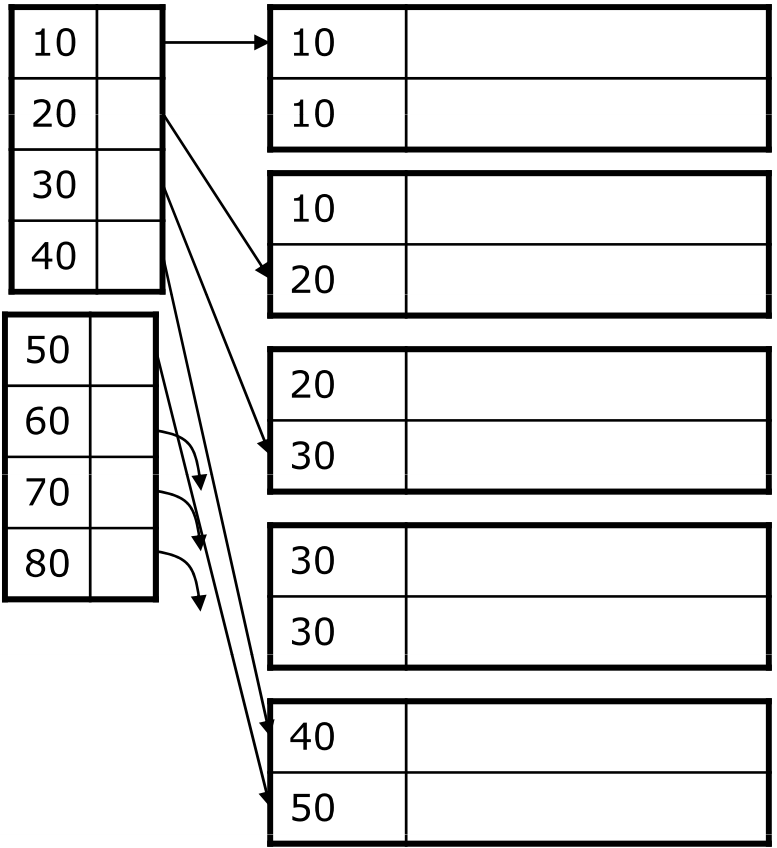
\includegraphics[scale=0.23]{img/Index_NonKey_Primary-Simple-1.png}
\end{column}
\begin{column}{.67\textwidth}
\begin{itemize}
\item Nur ein Feld-Adress-Paar $(K,P)$ je Schl\"usselwert $K$. 
\item Pointer $P$ zeigt auf erste Seite, die Datensatz mit Feld-Wert $K$ enth\"alt  
\item Weitere Datens\"atze mit Feld-Wert $K$ folgen direkt in der Seite oder in nachfolgenden Seiten.
\end{itemize}
\end{column}
\end{columns}
\end{frame}

\begin{frame}{\insertsection}
\framesubtitle{\insertsubsection}
\structure{\textbf{Einfacher Prim\"arindex auf Nicht-Schl\"ussel-Feldern -- Sparse Index (Variante 1)}}
\\[4pt]
\begin{columns}[T]
\begin{column}{.33\textwidth}
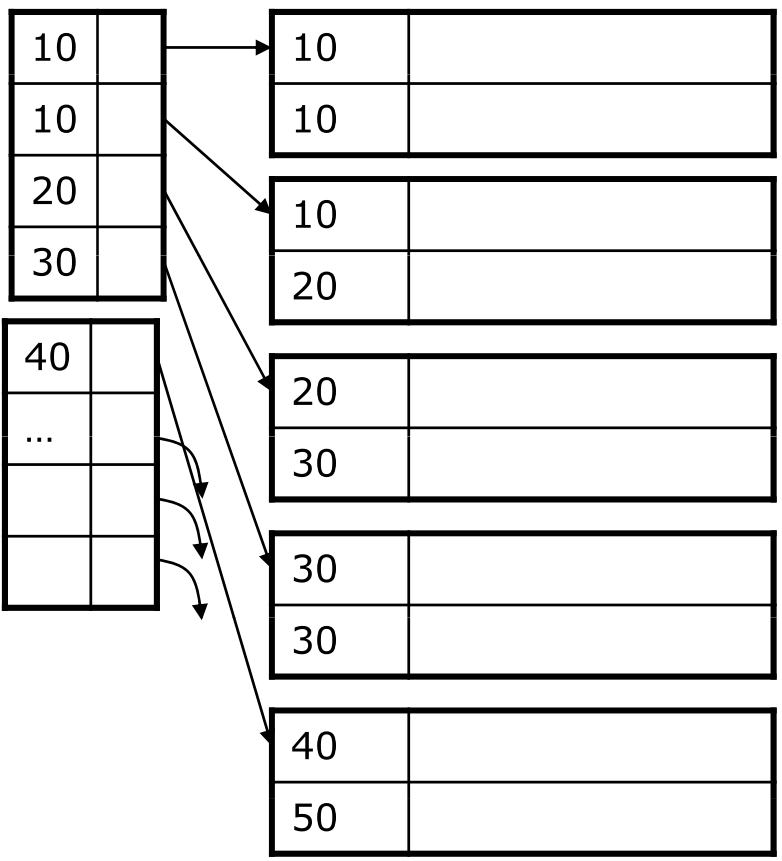
\includegraphics[scale=0.23]{img/Index_NonKey_Primary-Simple-2.png}
\end{column}
\begin{column}{.67\textwidth}
\begin{itemize}
\item Ein Feld-Adress-Paar $(K,P)$ je Seite. 
\item Feld-Wert $K$ ist der Wert des ersten Datensatzes in der Seite bei Adresse $P$.  
\item Weitere Datens\"atze mit Feld-Wert $K$ folgen direkt in der Seite oder in nachfolgenden Seiten.
\end{itemize}
\end{column}
\end{columns}
\end{frame}

\begin{frame}{\insertsection}
\framesubtitle{\insertsubsection}
\structure{\textbf{Einfacher Prim\"arindex auf Nicht-Schl\"ussel-Feldern -- Sparse Index (Variante 2)}}
\\[4pt]
\begin{columns}[T]
\begin{column}{.33\textwidth}
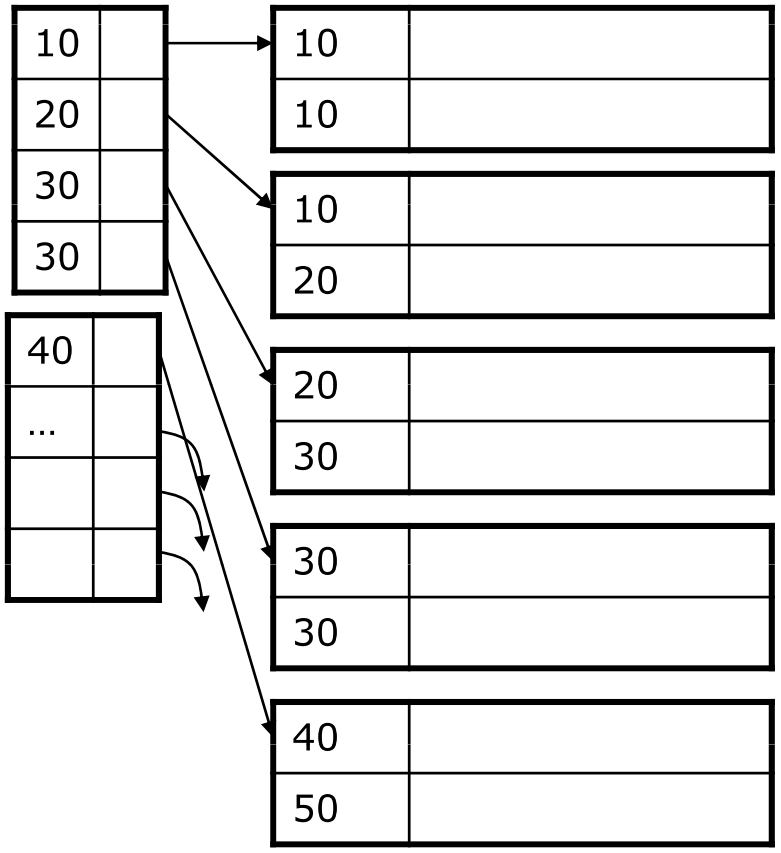
\includegraphics[scale=0.23]{img/Index_NonKey_Primary-Simple-3.png}
\end{column}
\begin{column}{.67\textwidth}
\begin{itemize}
	\item Erstes Feld-Adress-Paar $(K_1,P_1)$ im Index: $K_1$ kleinster Feld-Wert der Relation, Pointer $P_1$ auf erste Datenseite
	der Relation.
	\item Weitere Feld-Adress-Paare $(K,P)$ im Index: 
	\begin{itemize}
		\item Pointer $P =$ Adresse der nachfolgenden Datenseite. 
		\item Hat diese Datenseite neue Feld-Werte, dann setze $K =$ kleinster \textit{neuer} Feld-Wert in der Datenseite
		\item Sonst setze $K =$ aktueller Wert
		\item F\"uge $(K,P)$ zu Index hinzu
	\end{itemize}
\end{itemize}
%\nowrite{ 
%	% Pseudocode
%	K = K1 							# kleinster Feldwert in der Relation 
%	D = [P1, ..., Pn]		# alle Adressen der Datenseiten (geordnet)
%	Index = ((K1,P1))		# erster Eintrag im Index 
%	
%	for j in (1,n)			
%	if Seite(Pj) enthält Satz mit Feldwert > K
%	K = kleinster neuer Feldwert aus Seite(Pj)
%	Index.add((K,Pj))	
%}
\end{column}
\end{columns}
\end{frame}

\begin{frame}{\insertsection}
\framesubtitle{\insertsubsection}
\structure{\textbf{Einfache Prim\"arindizes}}
\\[4pt]
\structure{Noch ausstehende Betrachtungen:}
\begin{itemize}
	\item Suche von Datens\"atzen mit Hilfe des Index
	\item \"Anderungsoperationen (insert, update, delete) auf den Datens\"atzen mit Hilfe des Index
	\item Laufzeituntersuchung
\end{itemize}
\end{frame}

\subsection{Einfacher Sekund\"arindex}

\begin{frame}{\insertsection}
\framesubtitle{\insertsubsection}
\structure{\textbf{Einfacher Sekund\"arindex}}
\\[4pt]
\begin{columns}[T]
	\begin{column}{.33\textwidth}
		\includegraphics[scale=0.25]{img/Index_Secondary-Simple-1.png}
	\end{column}
	\begin{column}{.67\textwidth}
		\begin{itemize}
			\item Index-Feld(er) kein Schl\"ussel in der Relation.
			\item Index-Feld-Pointer-Paare im Index sortiert nach Index-Feld.
			\item Mehrere Index-Feld-Pointer-Paare mit gleichen Index-Feld-Werten m\"oglich.
			\item Datens\"atze in den Seiten nicht nach den zugeh\"origen Feldern sortiert.
		\end{itemize}
	\end{column}
\end{columns}
\end{frame}

\begin{frame}{\insertsection}
\framesubtitle{\insertsubsection}
\structure{\textbf{Einfacher Sekund\"arindex} -- Indirektion durch Buckets}
\\[4pt]
\begin{columns}[T]
	\begin{column}{.33\textwidth}
		\includegraphics[scale=0.22]{img/Index_Secondary-Simple-2.png}
	\end{column}
	\begin{column}{.64\textwidth}
		\begin{itemize}
			\item Index-Feld-Pointer-Paare mit Pointer auf Buckets (sequentielle, ggf.~ver-pointerte Bl\"ocke)
			\item Buckets enthalten Adressen der Seiten mit den Datens\"atze der entsprechenden Feld-Werte
			\pause
			\item Vorteile
			\begin{itemize}
				\item Speicherplatzsparend, wenn Index-Feld-Werte {gro\ss} oder mehrfach vorhanden.
				\item Bestimmte Anfragen direkt durch Buckets beantwortbar: 
				Selektionen als Schnittmenge der zugeh\"origen Buckets
			\end{itemize}
			%\item Nachteil: Weitere Indirektion und Verwaltung der Struktur.
		\end{itemize}	
	\end{column}
\end{columns}
\end{frame}

\begin{frame}{\insertsection}
\framesubtitle{\insertsubsection}
\structure{\textbf{Einfacher Sekund\"arindex}}
\begin{figure}
	\includegraphics[width=320pt]{img/SecondaryIndex.pdf}
	\caption{Secondary Index auf einem sekundären Schlüsselattribut}
\end{figure}
\end{frame}

\begin{frame}{\insertsection}
\framesubtitle{\insertsubsection}
\structure{\textbf{Einfacher Sekund\"arindex}}
\begin{figure}
\includegraphics[width=320pt]{img/SecondaryIndex2.pdf}
\caption{Secondary Index auf einem sekundären Nicht-Schlüsselattribut}
\end{figure}
\end{frame}

\begin{frame}{\insertsection}
\framesubtitle{\insertsubsection}
\structure{\textbf{Einfacher Sekund\"arindex} -- Suche ohne Sekund\"arindex}
\begin{itemize}
\item Datei mit $30.000$ Datens\"atzen
\item Block-Größe: $1024$ Bytes
\item Datensatz-Länge: $100$ Bytes (Fixed)
\item Blockorganisation: Unspanned
\item Die Datendatei weist keine Sortierung anhand des Sekundär-Attributes auf.
\end{itemize}
\pause
\abs
Rechnung für direkte Suche nach Datensatz in Datendatei ohne Sekund\"arindex:
\begin{itemize}
\item $bfr=\left \lfloor\frac{1024}{100}\right\rfloor = 10, \Longrightarrow$ es werden $\left\lceil\frac{30000}{10}\right\rceil = 3000$ 
Datenbl\"ocke für die Speicherung benötigt
\item Sequentielle Suche auf der Datendatei im Durchschnitt: $\frac{3000}{2} = \mathbf{1500}$ \textbf{Blockzugriffe}
\end{itemize}
\end{frame}

\begin{frame}{\insertsection}
\framesubtitle{\insertsubsection}
\structure{\textbf{Einfacher Sekund\"arindex} -- Suche mit Sekund\"arindex}
\begin{itemize}
	\item Block-Größe: $1024$ Bytes
	\item Index-Feld-Länge: $9$ Bytes (Unique)$\quad$/$\quad$ Pointer-Länge: $6$ Bytes
	\item Somit: Sekund\"arindex-L\"ange: $15$ Bytes
	\item Index-Eintrag je Datenblock der Datendatei (unsortiert) $\Rightarrow$ 30.000 Index-Datens\"atze
\end{itemize}
\pause
\ \\[4pt]
Suche nach Datensatz mit Sekund\"arindex:
\begin{itemize}
	\item $bfr_I=\left \lfloor\frac{1024}{15}\right\rfloor = 68 \Rightarrow\left\lceil\frac{30000}{68}\right\rceil = 442$ 
	Indexbl\"ocke ben\"otigt
	\pause
	\item Bin\"are Suche in Index-Datei: $\log_2 442 \approx \mathbf{9}$ \textbf{Blockzugriffe}
	\item Weiterer Blockzugriff, um passenden Datensatz aus Datendatei zu holen
\end{itemize}
\pause
\ \\[4pt]
\textbf{1500 Blockzugriffe ohne Index gegen\"uber 10 Blockzugriffen mit Sekund\"arindex}
\end{frame}

%%%%%%%%%%%%%%%%%%%%%%%%%%%%%%%%%%%%%%%%%%%%%%%
% Clustered Index vorerst weglassen --> B-Bäume
%%%%%%%%%%%%%%%%%%%%%%%%%%%%%%%%%%%%%%%%%%%%%%%
\nowrite{ 
\subsection{Clustered Index}
%
\begin{frame}{\insertsection}
	\framesubtitle{\insertsubsection}
	\structure{Eigenschaften des Clustered Index:}
	\begin{itemize}
		\item Ein Clustered Index ist ebenfalls eine sortierte Datei mit Records fixer Länge
		\item Er wird über einem Sortierfeld einer Datendatei gebildet. Das Sortierfeld muss jedoch \textit{nicht} eindeutig sein
		\item Jeder Record besteht ebenfalls aus zwei Feldern: 
			\begin{itemize}
					\item Das erste Feld ist vom selben Datentyp wie das Sortierfeld der Datendatei
					\item Das zweite Feld ist ein Pointer auf einen Disk Block, in dem der Record liegt
				\end{itemize}
		\structure{Der Clustered Index besitzt somit die gleiche Struktur wie der Primary Index}
		
		\alert{Aber: An Stelle eines Eintrages pro Disk Block enthält der Clustered Index nun einen Eintrag für jeden unterschiedlichen Wert des Sortierfeldes! Auch der Clustered Index ist ein \textit{sparse Index}}.	
	\end{itemize}
\end{frame}
%
\begin{frame}{\insertsection}
	\framesubtitle{\insertsubsection}
	\begin{figure}
	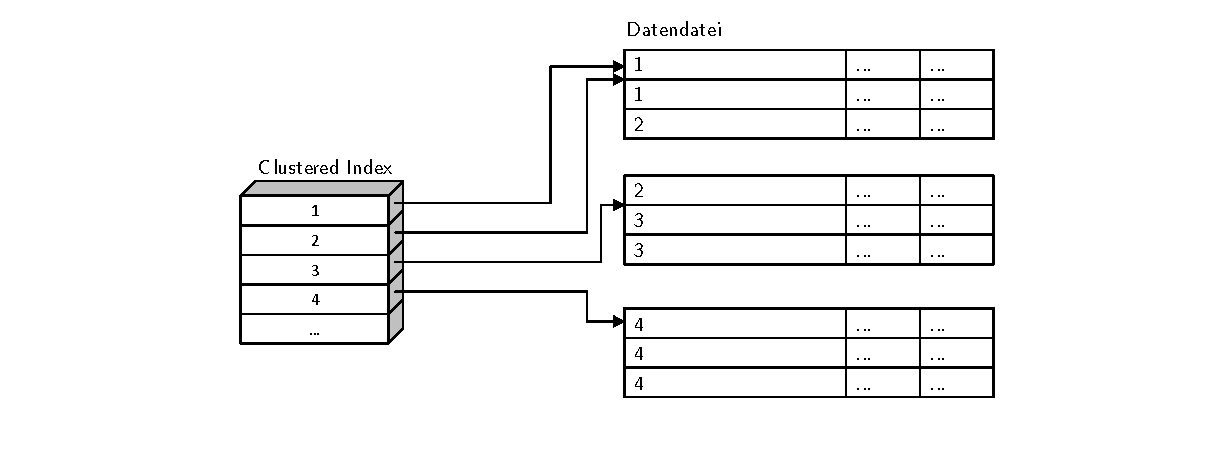
\includegraphics[width=350pt]{img/ClusteredIndex.pdf}
	\caption{Clustered Index mit Block-Pointer auf Datendatei-Blöcke}
	\end{figure}
\end{frame}
%
\begin{frame}{\insertsection}
	\framesubtitle{\insertsubsection}
	\structure{Einfüge-Operationen:}
	\begin{itemize}
	\item Die bisherige Variante des Clustered Index kann nicht gut mit Einfügeoperationen umgehen (gleiche Problematik wie bei Primary Index)
	\item Daher gibt es für den Clustered Index eine Alternative: 
	\begin{itemize}
		\item Da zwar eine Sortierung vorliegt, aber keine Eindeutigkeit der Attributwerte, kann mit einer Variante der Overflow-Listen gearbeitet werden.
		\item Jeder Block beinhaltet nur einen Index-Wert in den Records
		\item Wird ein Block durch eine Einfüge-Operation zu voll, so wird ein Block Pointer am Ende eingefügt und der Block damit künstlich vergrößert.
		\item Ein \texttt{null}-Pointer zeigt an, dass es keine weiteren Einträge mit dem Attributwert mehr gibt.
	\end{itemize}
	\end{itemize}
\end{frame}
%
\begin{frame}{\insertsection}
	\framesubtitle{\insertsubsection}
	\begin{figure}
		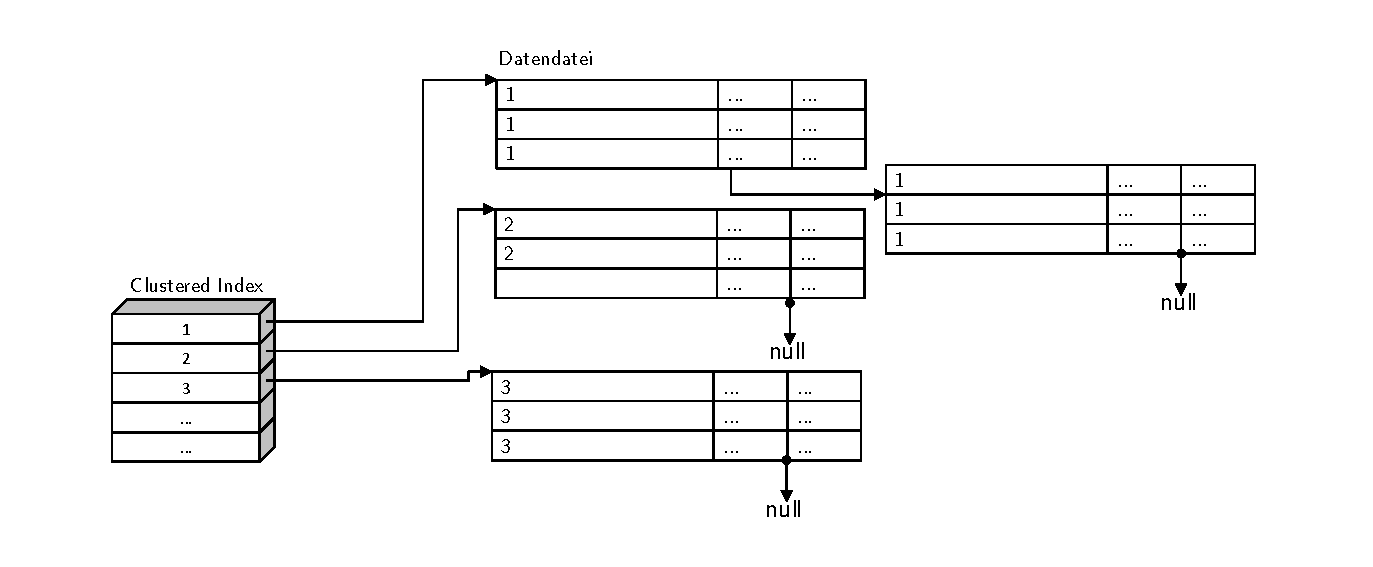
\includegraphics[width=370pt]{img/ClusteredIndex2.pdf}
	\caption{Alternative des Clustered Index zum Auflösen der Einfügeproblematik}
	\end{figure}
\end{frame}
}
%%%%%%%%%%%%%%%%%%%%%%
% Ende Clustered Index 
%%%%%%%%%%%%%%%%%%%%%%

\section{Mehrstufiger Index}

\begin{frame}{\insertsection}
\framesubtitle{\insertsubsection}
\structure{\textbf{Idee und Konzeption}}\\[4pt]
\begin{columns}[T]
	\begin{column}{.5\textwidth}
		\begin{itemize}
			\item Auch ein Index kann gro\ss\ werden.
			\begin{itemize}
				\item Kostet zus\"atzlichen I/O und Speicher
			\end{itemize}
			\item Idee: Zweiten Index \"uber den ersten Index legen
			\item Zweiter Index nur als dünn besetzter Index sinnvoll. Warum?\\[10pt]
			\pause
			\item Im Prinzip auch dritte, vierte, etc.~Ebene denkbar. 
			\item Mehrstufigkeit bringt weitere Effizienz. \textbf{Aber:} B-B\"aume besser geeignet, 
			da inh\"arent mehrstufig -- siehe sp\"ater
		\end{itemize}
	\end{column}
	\onslide
	\begin{column}{.45\textwidth}
		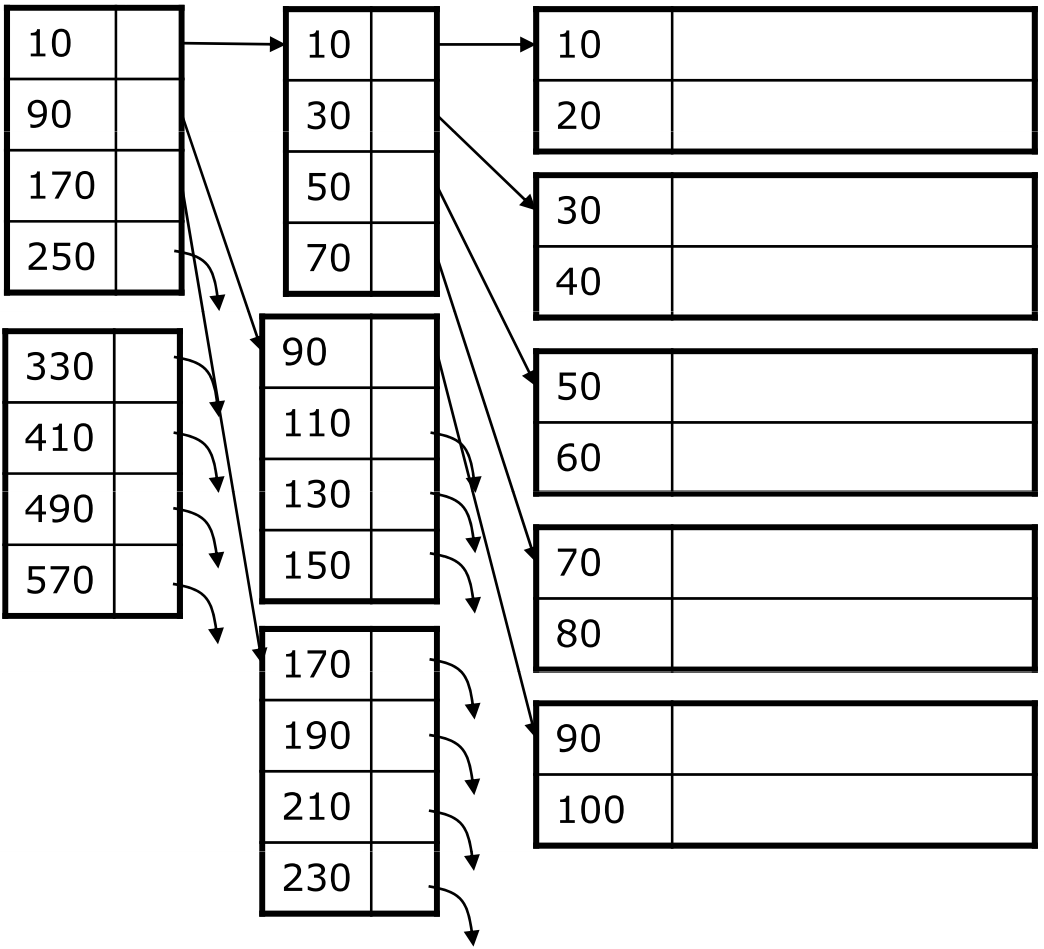
\includegraphics[scale=0.25]{img/Index_Multilevel.png}
	\end{column}
\end{columns}
\end{frame}

\begin{frame}{\insertsection}
\framesubtitle{\insertsubsection}
\structure{\textbf{Idee und Konzeption}}\\[4pt]
\begin{figure}
\includegraphics[width=350pt]{img/MultiIndex.pdf}
\caption{Mehrstufiger Index}
\end{figure}
\end{frame}

\begin{frame}{\insertsection}
\framesubtitle{\insertsubsection}
\structure{\textbf{Schnellerer und effizienterer Zugriff durch mehrstufigen Index}}\\[4pt]
\begin{itemize}
%\item Ersetze bin\"are Suche durch $m$-\"are Suche mit $m> 2$.
%\end{itemize}
%\begin{block}{Begr\"undung}
%	\begin{itemize}
%		\item Sei 
%	\end{itemize}
%\end{block}
\item Bisher: Sortierte Indizes nutzen binäre Suchalgorithmik.
\item Halbierung des Suchraums in jedem Suchschritt. Reduktionsfaktor $b=2$.
\item Resultierende Komplexitätsklasse: $O(\log_2 n)$ (Logarithmus zur Basis $b=2$).
%\item Der Logarithmus zur Basis 2 trägt der Halbierung des Suchraums Rechnung. Man spricht auch vom Fan-Out $fo=2$.
\end{itemize}
\pause
\ \\[4pt]
Wir werden zeigen: 
\begin{itemize}
\item Mehrstufige Indizes erlauben schnellere Verkleinerung des Suchraums je Suchschritt.
\item Reduktionsfaktor $b>2$ f\"ur schnellere Verkleinerung des Suchraums.
\item Obere Schranke f\"ur Reduktionsfaktor: $b\le bfr_\mathrm{\,I}=\left \lfloor\frac{B}{r}\right\rfloor$, mit $B=$ Blockl\"ange und $r=$ 
L\"ange der Index-Tupel. 
\item Resultierende Komplexitätsklasse: $O(\log_b n)$ (Logarithmus zur Basis $b>2$).
\end{itemize}
%\alert{Gesucht ist daher eine Index-Datei mit $fo = bfr$}
\end{frame}

%\begin{frame}{\insertsection}
%\framesubtitle{\insertsubsection}
%\structure{Konstruktion eines mehrstufigen Index mit Reduktionsfaktor $b=bfr_\mathrm{\,I}$}
%\begin{itemize}
%\item Die erste Stufe ist ein Index f\"ur die Datens\"atze. 
%\item Die zweite Stufe ist ein Index f\"ur den Index der ersten Stufe.
%\item Jede weitere Stufe ist ein Index für die vorherige Index-Stufe.
%\item Alle Indizes sind geordnet in den (eindeutigen) Suchfeldern.
%\end{itemize}
%\end{frame}

\begin{frame}{\insertsection}
\framesubtitle{\insertsubsection}
\structure{\textbf{Konstruktion eines mehrstufigen Index mit Reduktionsfaktor $b=bfr_\mathrm{\,I}$}}\\[4pt]
\begin{columns}[T]
\begin{column}{.5\textwidth}
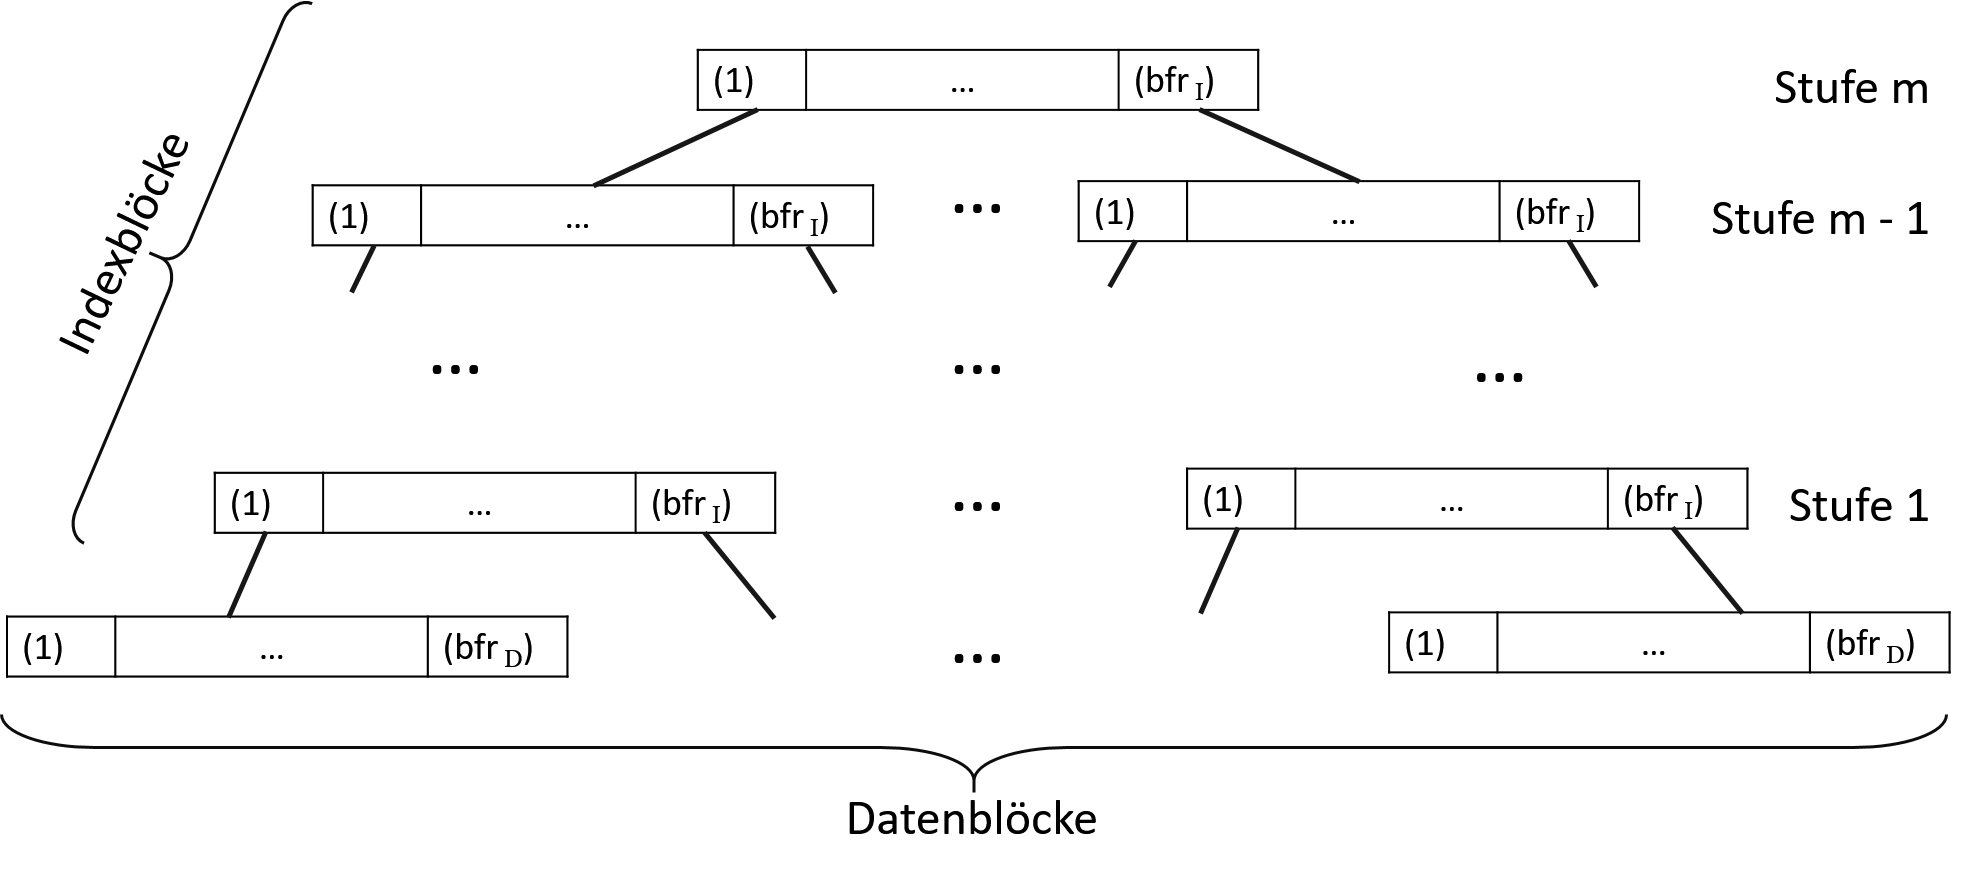
\includegraphics[height=.66\textwidth, width=1.05\textwidth]{img/Index_Multilevel_Zugriffe.png}
\end{column}
\begin{column}{.51\textwidth}
\begin{itemize}
\item Mehrstufiger Index mit $m$ Stufen. 
\item Jeder Indexblock hat Blocking Factor $bfr_\mathrm{\,I}$.
\item Damit $(bfr_\mathrm{\,I})^m$ Datenbl\"ocke adressierbar.
\ \\[8pt]\pause
\item Datenbl\"ocke mit Blocking Factor $bfr_\mathrm{\,D}$.
\item Maximal erreichbare Anzahl Datens\"atze: 
\begin{itemize}
	\item $(bfr_\mathrm{\,I})^m\cdot bfr_\mathrm{\,D}$ Datens\"atze (sortiert)\\[4pt]
	\item $(bfr_\mathrm{\,I})^m$ Datens\"atze (unsortiert)
\end{itemize}
\ \\[8pt]\pause
\item F\"ur jeden Datensatz werden $m+1$ Blockzugriffe ben\"otigt: $m$ Indexbl\"ocke und $1$ Datenblock.
\end{itemize}
%	Ein mehrstufiger Index auf der ersten Stufe mit $n$ Index-Blöcken kann durch $m$ Ebenen , wobei gilt 
%	$m=\left\lceil\log_{bfr_\mathrm{\,I}}n\right\rceil$.
\end{column}
\end{columns}
\end{frame}

\begin{frame}{\insertsection}
\framesubtitle{\insertsubsection}
\structure{\textbf{Mehrstufiger Index mit Reduktionsfaktor $b=bfr_\mathrm{\,I}$}}\\[4pt]
\structure{Beispiel}
\begin{itemize}
	\item Block-Gr\"o\ss e: $B=1024$ Bytes
	\item 30.000 Datens\"atze, Datensatzl\"ange: $R=100$ Bytes, Daten in Datendatei (\textbf{unsortiert}).
	\item Sekund\"arindex: Schl\"usselfeld $9$ Bytes, Pointer $6$ Bytes. Somit Index-Datensatz $15$ Bytes.
\end{itemize}
\pause
\ \\[4pt]
Berechnung Anzahl Zugriffe bei Suche nach Datensatz:
\begin{itemize}
	\item Index Blocking Factor: $bfr_\mathrm{\,I}=\left \lfloor\frac{1024}{15}\right\rfloor = 68$.
	\item $\left\lceil\frac{30.000}{68}\right\rceil = 442$ Bl\"ocke f\"ur Index der ersten Stufe ben\"otigt.
	\item $\left\lceil\frac{442}{68}\right\rceil = 7$ Bl\"ocke f\"ur Index der zweiten Stufe ben\"otigt.
	\item $\left\lceil\frac{7}{68}\right\rceil = 1$ Block f\"ur Index der dritten Stufe ben\"otigt.
\end{itemize}
\ \\[4pt]
\pause
1 Blockzugriff je Index-Stufe und 1 Datenblockzugriff $\Rightarrow$ \textbf{4 Blockzugriffe} insgesamt 
\pause\nl\textbf{Wieviele Zugriffe im sortierten Fall?}
\end{frame}

\section{B-Bäume}
\subsection{Definitionen}

\begin{frame}{\insertsection}
\framesubtitle{\insertsubsection}
\begin{columns}[T]
	\begin{column}{.6\textwidth}
		\begin{definition}[Baum]
			Ein Baum ist ein zusammenh\"angender Graph aus Knoten und Kanten, der keine Zykel enth\"alt. 
			Au\ss erdem hat der Baum einen ausgezeichneten Wurzelknoten $w$. 
		\end{definition}
	\end{column}
	\begin{column}{.3\textwidth}
		\includegraphics[scale=0.47]{img/Tree-Sample.png}
	\end{column}
\end{columns}
\end{frame}

\begin{frame}{\insertsection}
\framesubtitle{\insertsubsection}
\begin{columns}
\begin{column}{.6\textwidth}
	\begin{block}{\textbf{Notation}}
		\begin{itemize}
			\item Wurzelweg: Weg zwischen Wurzel $w$ und einem Knoten $k$. 
			\begin{itemize}
				\item \normalsize{Kanonische Richtung: $w\rightarrow k$}
			\end{itemize}
			\item Kante zwischen zwei Knoten $p$ und $q$ dadurch gerichtet: $p\rightarrow q$ oder $(p,q)$.
			\begin{itemize}
				\item \normalsize{$p =\,$Elternknoten von $q$, $q =\,$Kindknoten von $p$}
			\end{itemize}		
			\item Blattknoten: Endknoten $b$ eines Wurzelweges maximaler L\"ange.		
			\item Innerer Knoten $\ne$ Wurzel und $\ne$ Blattknoten.
		\end{itemize}
	\end{block}
\end{column}
\begin{column}{.3\textwidth}
	\includegraphics[scale=0.47]{img/Tree-Sample-Details.png}
\end{column}
\end{columns}
\end{frame}

\begin{frame}{\insertsection}
\framesubtitle{\insertsubsection}
\begin{columns}
	\begin{column}{.6\textwidth}
		\begin{definition}[Balancierter Baum]
			In einem balancierten Baum sind alle Wege von der Wurzel zu den Blattknoten gleich lang. 
		\end{definition}
	\end{column}
	\begin{column}{.3\textwidth}
		\includegraphics[scale=0.47]{img/Tree-BalanceTree-Sample.png}
	\end{column}
\end{columns}
\end{frame}

\begin{frame}{\insertsection}
\framesubtitle{\insertsubsection}
\structure{Suchbäume}
\begin{columns}
	\begin{column}{.48\textwidth}
		\begin{itemize}
			\item Suchbäume unterst\"utzen die Suche eines bestimmten Datensatzes/Blocks/Seite.
			\item Ein Knoten eines Suchbaums entspricht einer Seite (Block) des Speichers.
			\pause
			\ \\[12pt]
			\item Geeignete Suchb\"aume zur Verwendung als Index:
			\begin{itemize}
				\item {\normalsize $B$-B\"aume}
				\item {\normalsize $B^+$-B\"aume}
				\item {\normalsize $B^\star$-B\"aume}
			\end{itemize}
		\end{itemize}
	\end{column}
	\onslide
	\begin{column}{.58\textwidth}
		\begin{figure}
			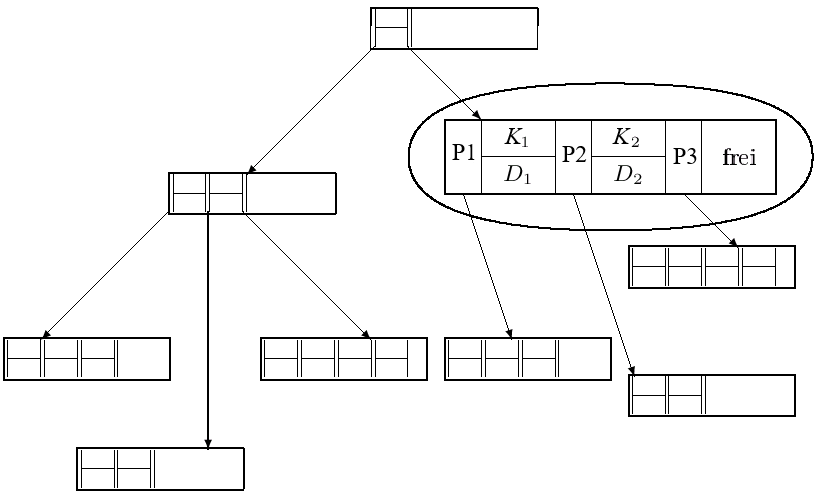
\includegraphics[scale=0.39]{img/BTree-1.png}
			\\[-10pt]\caption{Suchbaum (nach \cite{KE15})}
		\end{figure}
	\end{column}
\end{columns}
\end{frame}

\nowrite{ 
%%%%%%%%%%%%%%%%%%%%%%%%%%%%%%%%%%%%%%%%%%%%%%%%%%%%%%%%%%%%%%%%%
\begin{frame}{\insertsection}
\framesubtitle{\insertsubsection}
\begin{columns}
	\begin{column}{.65\textwidth}
		\begin{definition}[B-Baum der Ordnung $k$]
			B-Baum der Ordnung $k$ ist balancierter Suchbaum mit:
			\begin{itemize}
				\item Jeder Knoten enth\"alt $n$ Index-Tupel $(K_i,D_i)_{1\le i\le n}$ und $n+1$ Pointer $(P_j)_{1\le j\le n+1}$ 
				auf die Kindknoten.
				\begin{itemize}
					\item Wurzel: $1\le n \le 2k$. Sonstige Knoten: $k\le n \le 2k$.
					\item Indextupel liegen sortiert in Index-Werten $S_i$ vor.
					\item $D_i$: Datensatz mit Feldwert $S_i$ oder Pointer auf Block.
				\end{itemize}
				\pause
				\item $P_1$ zeigt auf Kindknoten mit Index-Werten $K < K_1$
				\item $P_i$ zeigt auf Kindknoten mit Index-Werten $K_{i} < K < K_{i+1}$ f\"ur $1\le i\le n-1$
				\item $P_{n+1}$ zeigt auf Kindknoten mit Index-Werten $K > K_n$
				\item In Blattknoten sind alle Pointer \texttt{null}
			\end{itemize}
		\end{definition}
	\end{column}
	\onslide
	\begin{column}{.34\textwidth}
		\begin{figure}
			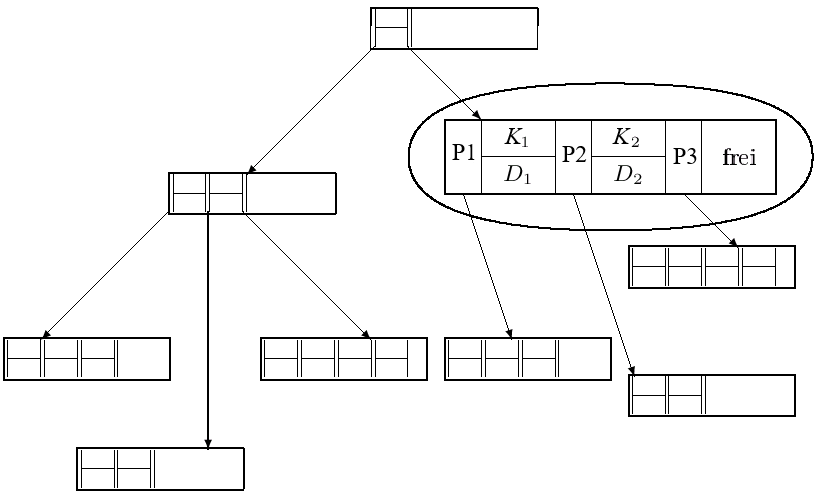
\includegraphics[scale=0.255]{img/BTree-1.png}
		\end{figure}
	\end{column}
\end{columns}
\end{frame}
%%%%%%%%%%%%%%%%%%%%%%%%%%%%%%%%%%%%%%%%%%%%%%%%%%%%%%%%%%%%%%%%%
}

\begin{frame}{\insertsection}
\framesubtitle{\insertsubsection}
\begin{columns}
	\begin{column}{.65\textwidth}
		\begin{definition}[B-Baum der Ordnung $k$]
			\begin{itemize}
				\item Balancierter Suchbaum
				\item Jede Knoten enthält $n\le 2\,k$ sortierte Index-Tupel $(K_i,D_i)_{1\le i\le n}$\pause
				\item $D_i$ ist (Pointer auf) Datensatz mit Wert $K_i$\pause
				\item Nicht-Wurzelknoten enthält $n\ge k$ Index-Tupel\pause
				\item Nicht-Blatt-Knoten hat $n + 1$ Kindknoten $(N_j)_{1\le j \le n+1}$\pause
				\begin{itemize}
					\item $N_1$ enth\"alt Index-Tupel mit Werten $K < K_1$\pause
					\item $N_j$ enth\"alt Index-Tupel mit Werten $K_{j} < K < K_{j+1}$ f\"ur $1\le j\le n-1$\pause
					\item $N_{n+1}$ enth\"alt Index-Tupel mit Werten $K > K_n$
				\end{itemize}
			\end{itemize}
		\end{definition}
	\end{column}
	\onslide
	\begin{column}{.345\textwidth}
		\begin{figure}
			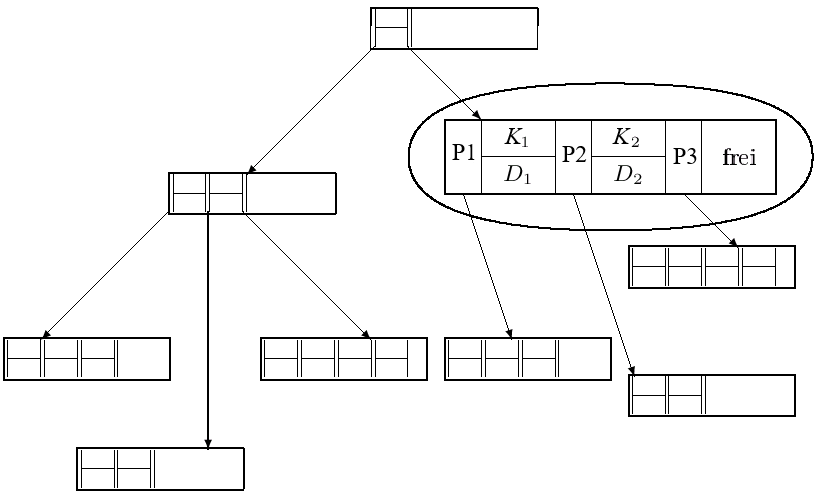
\includegraphics[scale=0.255]{img/BTree-1.png}
		\end{figure}
	\end{column}
\end{columns}
\end{frame}

\begin{frame}{\insertsection}
\framesubtitle{\insertsubsection}
\structure{Schematischer Aufbau eines Knotens eines B-Baums}
\begin{figure}
	\includegraphics[width=360pt]{img/tree1-adj.png}
	\caption{Nach \cite{EN10}}
\end{figure}
\end{frame}

\begin{frame}{\insertsection}
\framesubtitle{\insertsubsection}
\structure{Aufbau eines konkreten B-Baums}
\begin{figure}
\includegraphics[width=360pt]{img/tree2-adj.png}
\caption{Nach \cite{EN10}}
\end{figure}
\end{frame}

\subsection{Suchen, Einf\"ugen, L\"oschen}

\begin{frame}{\insertsection}
\framesubtitle{\insertsubsection}
\structure{Suchen in B-Baum}
\begin{enumerate}
	\item Suchknoten = Wurzelkonten
	\item\label{iter-b-search} Starte in Suchknoten die Suche nach Suchwert $S$ 
	\item Suche endet, wenn $S$ im Suchknoten enthalten ist $\Rightarrow$ Lade Datenblock/Lese Datensatz 
	\item Index-Eintrag/-Eintr\"age im Suchknoten ermitteln, dessen Kindknoten Wert $S$ überdeckt 
	\item Zeiger zum Kindknoten verfolgen und dessen Seite/Block laden
	\item F\"uhre Suche mit Suchknoten = Kindknoten ab Schritt \ref{iter-b-search} durch
	\item Ansonsten ist $S$ nicht im Baum enthalten
\end{enumerate}
\end{frame}

\begin{frame}{\insertsection}
\framesubtitle{\insertsubsection}
\structure{Beispiel: Suchen in B-Baum}
\abs
Suche: Werte $S=38,\,20,\,6$
\begin{figure}
	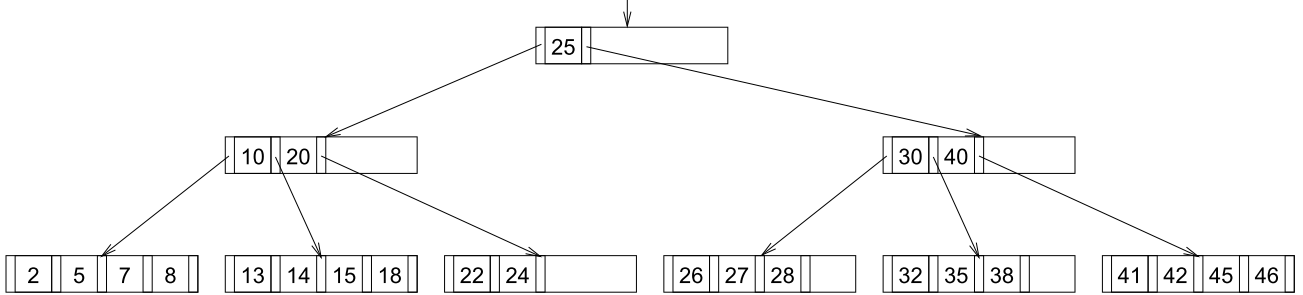
\includegraphics[scale=0.43]{img/BTree-Search.png}
\end{figure}
\end{frame}

\begin{frame}{\insertsection}
\framesubtitle{\insertsubsection}
\structure{Einf\"ugen von Index-Werten in einen B-Baum}
\begin{enumerate}
	\item Suche im Baum nach dem Index-Wert. Suche endet bei Einf\"ugestelle (Knoten).\pause
	\item F\"uge den Index-Wert dort ein, falls Wert nicht existiert und Knoten nicht gef\"ullt.\pause
	\item\label{full-node} Ist Knoten gef\"ullt und Index-Wert soll eingef\"ugt werden?\pause
	\begin{itemize}		
		\item	\"Uberf\"ulle den Knoten $\Rightarrow 2k+1$ Werte
		\item	Lege neuen Knoten auf gleicher Ebene an. Belege ihn mit Index-Werten, die rechts vom $(k+1)$.~Eintrag (Median)
		des \"uberf\"ullten Knotens liegen.
		\item	F\"uge Median im Elternknoten $E$ ein.
		\item	F\"uge Pointer zum neuen Knoten rechts des neuen Eintrags im Elternknoten $E$ ein.
	\end{itemize}\pause
	\item Ist Elternknoten $E$ jetzt überfüllt?\pause
	\begin{itemize}
		\item Handelt es sich bei $E$ um die Wurzel?
		\begin{itemize}
			\item Lege neuen Eltern-Wurzelknoten $E_0$ an.
			\item	F\"uge im neuen Wurzelknoten $E_0$ Pointer $P_1$ zu Knoten $E$ein.\pause
		\end{itemize}
		\item	Wiederhole Schritt \ref{full-node} mit Knoten $E$.
	\end{itemize}
\end{enumerate}
\end{frame}

\begin{frame}{\insertsection}
\framesubtitle{\insertsubsection}
\structure{Iteratives Einf\"ugen in B-Baum}
\begin{itemize}
	\item B-Baum wird mit einer Wurzel initialisiert.\pause
	\item Wurzel wird mit Index-Werten sortiert gef\"ullt. \pause
	\item Ist Wurzel voll, werden zwei Knoten und neuer Eltern-Wurzelknoten gebildet.\pause
	\item Mittlerer Index-Wert steigt in Elternwurzel auf, die anderen Werte werden auf Blatt-Kinder verteilt.\pause
	\item Weitere Werte werden in die Bl\"atter eingef\"ugt.\pause 
	\item Wird ein Blatt zu voll, wird es in zwei Blätter auf gleicher Ebene aufgespalten.\pause
	\item Der mittlere Index-Wert steigt in den Elternknoten auf.\pause 
	\item Ist Elternknoten voll, wird auch er gespalten. Das kann sich bis zur Wurzel fortsetzen.\pause 
\end{itemize}
\abs
\textbf{Folge:} Elemente werden \textit{stets} in Blättern eingefügt. Sie k\"onnen sp\"ater 'nach oben wandern'.
\end{frame}

\begin{frame}{\insertsection}
\framesubtitle{\insertsubsection}
\begin{center}
{\Huge DEMO}
% B-Baum-Insert-Delete-Demo.ppt - Einfügen zeigen (FF 1-59)
\end{center}
\end{frame}

\nowrite{
%%%%%%%%%%%%%%%%%%%%%%%%%%%%%%%%%%%%%%%%%%%%%%%%%%%%%%%%%
\begin{frame}{\insertsection}
\framesubtitle{\insertsubsection}
\structure{Einf\"ugen in einen B-Baum der Ordnung $1$: Werte 1,5,3}
\begin{figure}
 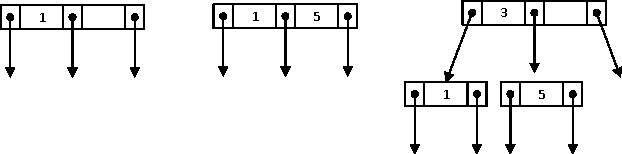
\includegraphics[width=350pt]{img/btree1.pdf}
	\end{figure}
\end{frame}
%
\begin{frame}{\insertsection}
\framesubtitle{\insertsubsection}
\structure{Einf\"ugen in einen B-Baum der Ordnung $1$: Werte 7,9}
\begin{figure}
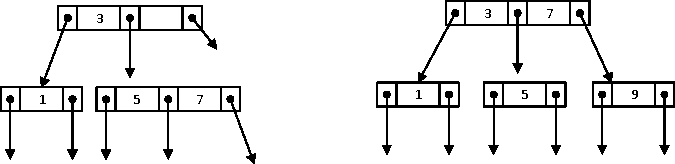
\includegraphics[width=350pt]{img/btree2.pdf}
\end{figure}
\end{frame}
%%%%%%%%%%%%%%%%%%%%%%%%%%%%%%%%%%%%%%%%%%%%%%%%%%%%%%%%%
}

\begin{frame}{\insertsection}
\framesubtitle{\insertsubsection}
\structure{Löschen in B-Bäumen setzt sich aus folgenden Operationen zusammen:}
\begin{itemize}
	\item \texttt{ROTATION}
	\item \texttt{MERGE}
	\item \texttt{DELETE} 
\end{itemize}
\end{frame}

\begin{frame}{\insertsection}
\framesubtitle{\insertsubsection}
\structure{Weitere Notation}\\[6pt]
Sei \texttt{N} Knoten. $m = k$, falls \texttt{N} Nicht-Wurzel oder $m=1$, falls \texttt{N} Wurzel
\begin{itemize}
\item \texttt{N <minimal>} : Knoten \texttt{N} hat genau $m$ Indexwert-Einträge 
\item \texttt{N <rich>}	:	Knoten \texttt{N} hat mehr als $m$ Indexwert-Einträge
\item \texttt{N <poor>}	:	Knoten \texttt{N} hat weniger als $m$ Indexwert-Einträge -- nicht B-Baum-konform
\end{itemize}
\end{frame}

\begin{frame}{\insertsection}
\framesubtitle{\insertsubsection}
\begin{figure}
	\centering	
	\includegraphics<1>[scale=0.35]{img/BTree-Rotation1.png}
	\includegraphics<2>[scale=0.35]{img/BTree-Rotation2.png}
	\includegraphics<3>[scale=0.35]{img/BTree-Rotation3.png}
\end{figure}
\structure{\texttt{ROTATION(N,N1)} : Verschiebe zyklisch Indexwerte von Knoten \texttt{N1} zu \texttt{N} \"uber Elternknoten}
\begin{enumerate}%[label=\roman*. , font=\small\ttfamily]
	\item \texttt{\small Knoten N <poor>, N1 Nachbarknoten von N (links bzw. rechts) <rich>}
	\pause
	\item \texttt{\small Verschiebe Wert K im Elternknoten P zwischen den Pointers nach N}
	\item \texttt{\small Verschiebe (gr\"o\ss ten bzw. kleinsten) Wert von N1 in die freigewordene Position in P}
\end{enumerate}
\end{frame}

\begin{frame}{\insertsection}
\framesubtitle{\insertsubsection}
\begin{figure}
\centering	
\includegraphics<1>[scale=0.35]{img/BTree-Merge1.png}
\includegraphics<2-3>[scale=0.35]{img/BTree-Merge2.png}
\includegraphics<4>[scale=0.35]{img/BTree-Merge3.png}
\end{figure}
\structure{\texttt{MERGE(N,N1)} : Führe Indexwerte von Knoten \texttt{N} und \texttt{N1} zusammen \"uber Elternknoten}
\begin{enumerate}
%[label=\roman*. , font=\small\ttfamily]
\item \texttt{\small Knoten N <poor>, Nachbarknoten N1 <minimal>}
\pause
\item \texttt{\small Füge Wert K im Elternknoten P zwischen den Pointers und die Knoten N und N1 zu einem Knoten zusammen}
\pause
\item \texttt{\small L\"oschen: Wert K im Elternknoten sowie leere Knoten mit Pointer}
\item \texttt{\small Einf\"ugen: Pointer von Elternknoten auf neuen Knoten}
\end{enumerate}
\end{frame}

\begin{frame}{\insertsection}
\framesubtitle{\insertsubsection}
\structure{\texttt{DELETE(N,K)} : L\"osche Indexwert \texttt{K} in Knoten \texttt{N}}
\begin{enumerate}
	%[label=\roman*. , font=\small\ttfamily]
	\item \texttt{\small Falls N Nicht-Blatt}
	\begin{enumerate}
		\item \texttt{\small Nullifiziere Wert K in N}
		\pause
		\item \texttt{\small Finde in Baum den n\"achst gr\"o\ss eren Wert K1 in einem Knoten L
			\nl	$\quad$	/* L ist Blatt. Warum? */}
		\pause
		\item \texttt{\small Kopiere K1 in die leer gewordene Position von K}
		\pause
		\item \texttt{\small DELETE(L,K1)}		
	\end{enumerate}
	\pause
	\item \texttt{\small Sonst (N ist Blatt)}
	\begin{enumerate}
		\item \texttt{\small Entferne K aus N}
		\pause
		\item \texttt{\small Falls N <poor>:}
		\pause
		\begin{itemize}
			\item \texttt{\small Falls Nachbarknoten N1 <rich> existiert: ROTATION(N,N1)}
			\pause
			\item \texttt{\small Sonst wähle einen Nachbarknoten N1 <minimal>: MERGE(N, N1)}
		\end{itemize}			
	\end{enumerate}	
	%\pause
	%\item \texttt{\small Lösche Knoten N und N1}
	%\item \texttt{\small Führe DELETE(P,N) im Elternknoten P durch, ersetze freigewordene Pointers durch Pointer auf Nn}
\end{enumerate}
\end{frame}

\begin{frame}{\insertsection}
\framesubtitle{\insertsubsection}
\structure{\texttt{DELETE(K)} : L\"osche Indexwert \texttt{K} in Baum}
\begin{enumerate}
\item \texttt{\small Finde Knoten N mit Indexwert K}
\item \texttt{\small	DELETE(N,K)}
\end{enumerate}
\end{frame}

\nowrite{
%%%%%%%%%%%%%%%%%%%%%%%%%%%%%%%%%%%%%%%%%%%%%%%%%%%%%%%%%%%%
\begin{frame}{\insertsection}
\framesubtitle{\insertsubsection}
\structure{Löschen in B-Bäumen:}
\begin{itemize}
	\item Ist zu l\"oschender Wert in Blatt, so kann er gel\"oscht werden.
	\item Es muss dabei auf die Minimalfüllung der Blätter geachtet werden.
	\item Ist das Blatt die Wurzel und diese danach leer, so kann die Wurzel gelöscht werden. B-Baum ist leer. 
	\item Ist das Blatt nicht die Wurzel und bleibt nach dem Löschen die Minimalfüllung erhalten, 
	so kann der Wert aus dem Blatt entfernt werden.	
	\item Ist zu löschender Wert in innerem Knoten, besitzt er zwei Nachfolgerknoten
	\begin{itemize}
		\item Der gelöschte Wert wird durch das Minimum des rechten bzw. das Maximum des linken Teilbaumes ersetzt. Der 
		Ersatzwert liegt dabei \textit{immer} in einem Blatt.
		\item Die Löschoperation in einem inneren Knoten wird dabei auf die Löschoperation in einem Blatt zurückgeführt
		\item \alert{Achtung: Auch jetzt müssen die B-Baum-Eigenschaften erhalten bleiben!}
	\end{itemize}
\item Ist die Minimalfüllung unterschritten, so muss die B-Baum-Eigenschaft durch die folgenden Operationen wiederhergestellt werden: 
\begin{itemize}
	\item Gibt es einen Nachbarn, der einen Wert verschieben könnte, so dass beide Knoten die Minimalfüllung nicht unterschreiten, so werden Werte verschoben (Rotation)
	\item Gibt es keinen solchen Nachbarn, so müssen zwei Knoten miteinander vereinigt werden (Merge)
\end{itemize}
\end{itemize}
\end{frame}
%%%%%%%%%%%%%%%%%%%%%%%%%%%%%%%%%%%%%%%%%%%%%%%%%%%%%%%%%%%%
}

\nowrite{
%%%%%%%%%%%%%%%%%%%%%%%%%%%%%%%%%%%%%%%%%%%%%%%%%%%%
\begin{frame}{\insertsection}
\framesubtitle{\insertsubsection}
\structure{Löschen in B-Bäumen:}
	\begin{itemize}
		\item Ist zu l\"oschender Wert in Blatt, so kann er gel\"oscht werden.
		\item Es muss dabei auf die Minimalfüllung der Blätter geachtet werden.
		\item Ist zu löschender Wert in innerem Knoten, besitzt er zwei Nachfolgerknoten
		\begin{itemize}
			\item Der gelöschte Wert wird durch das Minimum des rechten bzw. das Maximum des linken Teilbaumes ersetzt. Der 
			Ersatzwert liegt dabei \textit{immer} in einem Blatt.
			\item Die Löschoperation in einem inneren Knoten wird dabei auf die Löschoperation in einem Blatt zurückgeführt
			\item \alert{Achtung: Auch jetzt müssen die B-Baum-Eigenschaften erhalten bleiben!}
		\end{itemize}
	\end{itemize}
\end{frame}
%
\begin{frame}{\insertsection}
	\framesubtitle{\insertsubsection}
	\structure{Löschen in B-Baum-Blättern:}
	\begin{itemize}
		\item Ist das Blatt die Wurzel und ist diese leer, so kann die Wurzel gelöscht werden. Der B-Baum ist dann leer. 
		\item Ist das Blatt nicht die Wurzel und bleibt nach dem Löschen die Minimalfüllung erhalten, so kann der Wert aus dem Blatt entfernt werden.
		\item Ist die Minimalfüllung unterschritten, so muss die B-Baum-Eigenschaft durch die folgenden Operationen wiederhergestellt werden: 
		\begin{itemize}
			\item Gibt es einen Nachbarn, der einen Wert verschieben könnte, so dass beide Knoten die Minimalfüllung nicht unterschreiten, so werden Werte verschoben (Rotation)
			\item Gibt es keinen solchen Nachbarn, so müssen zwei Knoten miteinander vereinigt werden (Merge)
		\end{itemize}
		\end{itemize}
\end{frame}
%%%%%%%%%%%%%%%%%%%%%%%%%%%%%%%%%%%%%%%%%%%%%%%%%%%%
}

\nowrite{
%%%%%%%%%%%%%%%%%%%%%%%%%%%%%%%%%%%%%%%%%%%%%%%%%%%%
\begin{frame}{\insertsection}
	\framesubtitle{\insertsubsection}
	\structure{Rotation: Löschen von $r2$: }
\begin{figure}
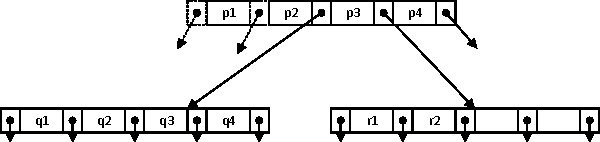
\includegraphics[width=350pt]{img/btreerotate.pdf}
	\caption{Löschen von $r2$ im B-Baum}
	\end{figure}
\end{frame}
%
\begin{frame}{\insertsection}
	\framesubtitle{\insertsubsection}
	\structure{Rotation: Löschen von $r2$: }
\begin{figure}
	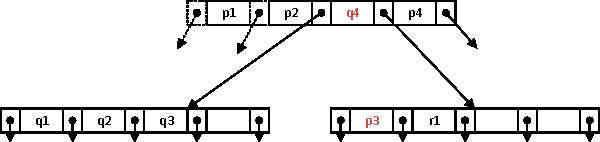
\includegraphics[width=350pt]{img/btreerotate2.pdf}
	\caption{Löschen von $r2$ im B-Baum}
	\end{figure}
\end{frame}
%
\begin{frame}{\insertsection}
	\framesubtitle{\insertsubsection}
	\structure{Merge: Löschen von $r2$: }
\begin{figure}
	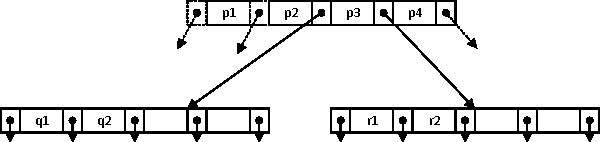
\includegraphics[width=350pt]{img/btreemerge.pdf}
	\caption{Löschen von $r2$ im B-Baum (Merge)}
	\end{figure}
\end{frame}
%
\begin{frame}{\insertsection}
	\framesubtitle{\insertsubsection}
	\structure{Merge: Löschen von $r2$: }
\begin{figure}
		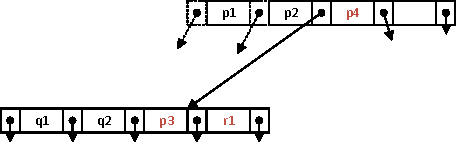
\includegraphics[width=350pt]{img/btreemerge2.pdf}
	\caption{Löschen von $r2$ im B-Baum (Merge)}
	\end{figure}
\end{frame}
%%%%%%%%%%%%%%%%%%%%%%%%%%%%%%%%%%%%%%%%%%%%%%%%%%%%
}

\begin{frame}{\insertsection}
\framesubtitle{\insertsubsection}
\begin{center}
	{\Huge DEMO}
	% B-Baum-Insert-Delete-Demo.ppt - Löschen zeigen (FF 61-Ende)    
\end{center}
\end{frame}

\begin{frame}{\insertsection}
\framesubtitle{\insertsubsection}
\structure{Weitere Eigenschaften von B-B\"aumen}
\abs
\begin{theorem}
Die H\"ohe $H$ eines B-Baums der Ordnung $k$ mit $n (>1)$ Indexwerten ist beschr\"ankt durch
\begin{equation*}
\log_{2k+1}(n-1) - 1 \le H \le \log_{k+1}\left(\frac{n+1}{2}\right) < \log_k(n)
\end{equation*}
\end{theorem}
\end{frame}

\begin{frame}{\insertsection}
\framesubtitle{\insertsubsection}
\structure{Weitere Eigenschaften von B-B\"aumen}
\abs
\begin{theorem}[Laufzeitverhalten]
Die Operationen Lesen, Einf\"ugen oder L\"oschen in einem B-Baum der Ordnung $k$ mit $n$ Indexwerten k\"onnen mit 
\begin{equation*}
\mathcal{O}\left(\log_{k}(n)\right)
\end{equation*}
Blockzugriffen durchgef\"uhrt werden.
\end{theorem}
\end{frame}

\begin{frame}{\insertsection}
\framesubtitle{\insertsubsection}
\structure{Beispiel}
\begin{itemize}
\item B-Baum der Ordnung $k=50$
\item B-Baum enth\"alt $n=1.000.000$ Index-Einträge 
\item Suchkomplexität: $O(\log_{k}n)$
\item Blockzugriffe $b$: 
$$b\le\left\lfloor\log_{50}(1.000.000)\right\rfloor=3$$	
\end{itemize}
\abs\pause
\begin{itemize}
\item B-Baum der Ordnung $k=50$ mit $1.000.000$ Index-Werten
\item Auffinden eines Wertes: max.~$3$ Knotenzugriffe (Seiten oder Bl\"ocke).
\item Weiterer Blockzugriff auf den eigentlichen Datensatz. 
\item Also: Insgesamt max.~$4$ Blockzugriffe.
\end{itemize} 
\end{frame}

\begin{frame}{\insertsection}
\framesubtitle{\insertsubsection}
\structure{Zusammenfassung}
\begin{itemize}
\item B-B\"aume sind balancierte Suchb\"aume, geeignet als Prim\"ar- oder Sekund\"arindex.
\item H\"ohe des Suchbaums, Zeitaufwand (Suchen, Einf\"ugen, L\"oschen): $\mathcal{O}\left(\log_{k}(n)\right)$.
\item B-Bäume sind dynamische Datenstrukturen
\begin{itemize}
	\item Ver\"andern sich zuerst stark
	\item Je mehr Einträge in B-Baum, umso stabiler
	\item Knotenfüllung dann ca. 70\%
\end{itemize}
\item Varianten von B-Bäumen:
\begin{itemize}
\item $B^+$-Bäume: Datenblock-Pointer nur in Blättern enthalten. Blätter als verkettete Liste angelegt.
\item $B^*$-Bäume: $B^+$-Bäume, deren Knoten mindestens zu $\frac{2}{3}$ gefüllt sein müssen.
\end{itemize}
\end{itemize}                                               
\end{frame}

\begin{frame}{\insertsection}
\framesubtitle{\insertsubsection}	
\begin{block}{\textbf{\"Ubungsaufgabe}}
Fügen Sie nacheinander die folgende Zahlenreihe (in der Reihenfolge) in einen B-Baum der Ordnung $k=2$ ein: 7,4,5,6,1,2,0,9,8
\end{block}
\end{frame}

\section{Hash-Basierter Index}

\begin{frame}{\insertsection}
\framesubtitle{\insertsubsection}	
\structure{Wiederholung Hash-Funktion}
\abs
Hash-Funktion bildet Wertebereich (Dom\"ane) $S$ auf Hash-Werte ab:
\begin{equation*}
h:S\to W,\quad s\mapsto h(s)\in W
\end{equation*}
In der Regel $\vert S\vert\gg \vert W\vert$, und somit $h$ \textbf{nicht} injektiv. 
\nl
Normalerweise $\vert W\vert<\infty$. Oft Dom\"ane $S$ potenziell unendlich {gro\ss}: $\vert S\vert=\infty$.
\abs
\pause
Einsatz von Hash-Funktionen in unterschiedlichen Kontexten: 
\begin{itemize}
	\item Kryptografische Hashfunktionen
	\item Prüfsummenberechnung
	\item Zuweisung von Speicher in Hash-Datei, Hash-basierter Index
\end{itemize}
\end{frame}

\begin{frame}{\insertsection}
\framesubtitle{\insertsubsection}	
\structure{Einf\"uhrung}
\begin{itemize}
\item Hash-basierte Indizes sind 'unschlagbar' bei SQL-Anfragen mit Gleichheitsbedingungen:
\abs
\ \ \ \ \ \ \texttt{SELECT * FROM TableT WHERE FieldF = "field value"}
\abs
Insbesondere: Equi-Joins, Nested Loop Joins, etc.
\item Hash-basierte Indizes bieten keine Unterstützung bei Bereichsanfragen.	
\end{itemize}
\pause
\begin{itemize}
\item Hash-basierte Indizes nutzen bei der Suche eines Datensatzes den Index-Wert $K$ direkt, 
unabhängig von den anderen Index-Werten. 
\item In B-Baum wird Datensatz-Adresse durch Vergleich des Index-Wertes $K$ mit anderen Index-Werten
in der Baumstruktur ermittelt.
\end{itemize}
\abs
\pause
Wichtige Varianten von Hash-basierten Indizes:
\begin{itemize}
\item Statisches Hashing
\item Erweiterbares (dynamisches) Hashing	
\end{itemize}	
\end{frame}

\subsection{Statisches Hashing}

\begin{frame}{\insertsection}
\framesubtitle{\insertsubsection}	
\structure{Konzept}
\begin{itemize}
\item Dateneintr\"age werden mittels Hash-Funktion in Buckets gesucht/einsortiert.
\item Bucket besteht aus Prim\"arseite und ggf.~weiteren ver-pointerten \"Uberlaufseiten.
\item Index besteht aus Bucket-Nummer und Pointer zu Prim\"arseite.
\end{itemize}
\begin{figure}[T]
\includegraphics<1>[scale=0.22]{img/Hash-stat-00.png}
\end{figure}
\end{frame}

\begin{frame}{\insertsection}
\framesubtitle{\insertsubsection}	
\structure{Wahl der Hash-Funktion}
\begin{itemize}
\item Da Hash-Funktion nicht injektiv, Kollisionen $h(k) = h(k')$ f\"ur Index-Werte $k\ne k'$ m\"oglich.
\item Somit Datens\"atze f\"ur $k$ und $k'$ in gleichen Buckets.  
\item Das ist erw\"unscht. Sonst genauso viele Buckets wie Index-Werte ben\"otigt!
\item Idealerweise: Hash-Funktion mit nahezu Gleichverteilung der Index-Werte \"uber Buckets. 
\end{itemize}
\abs
\pause
H\"aufig verwendete Hash-Funktion ist Division durch ganze Zahl $p$ mit Rest:
\begin{equation*}
h(s) \equiv s\mod p
\end{equation*}
Oft $p$ Primzahl, wodurch recht gute Gleichverteilung erzielt werden kann. 
\end{frame}

\begin{frame}{\insertsection}
\framesubtitle{\insertsubsection}	
\structure{Einf\"ugen eines Datensatzes}
\\[-8pt]
\begin{figure}
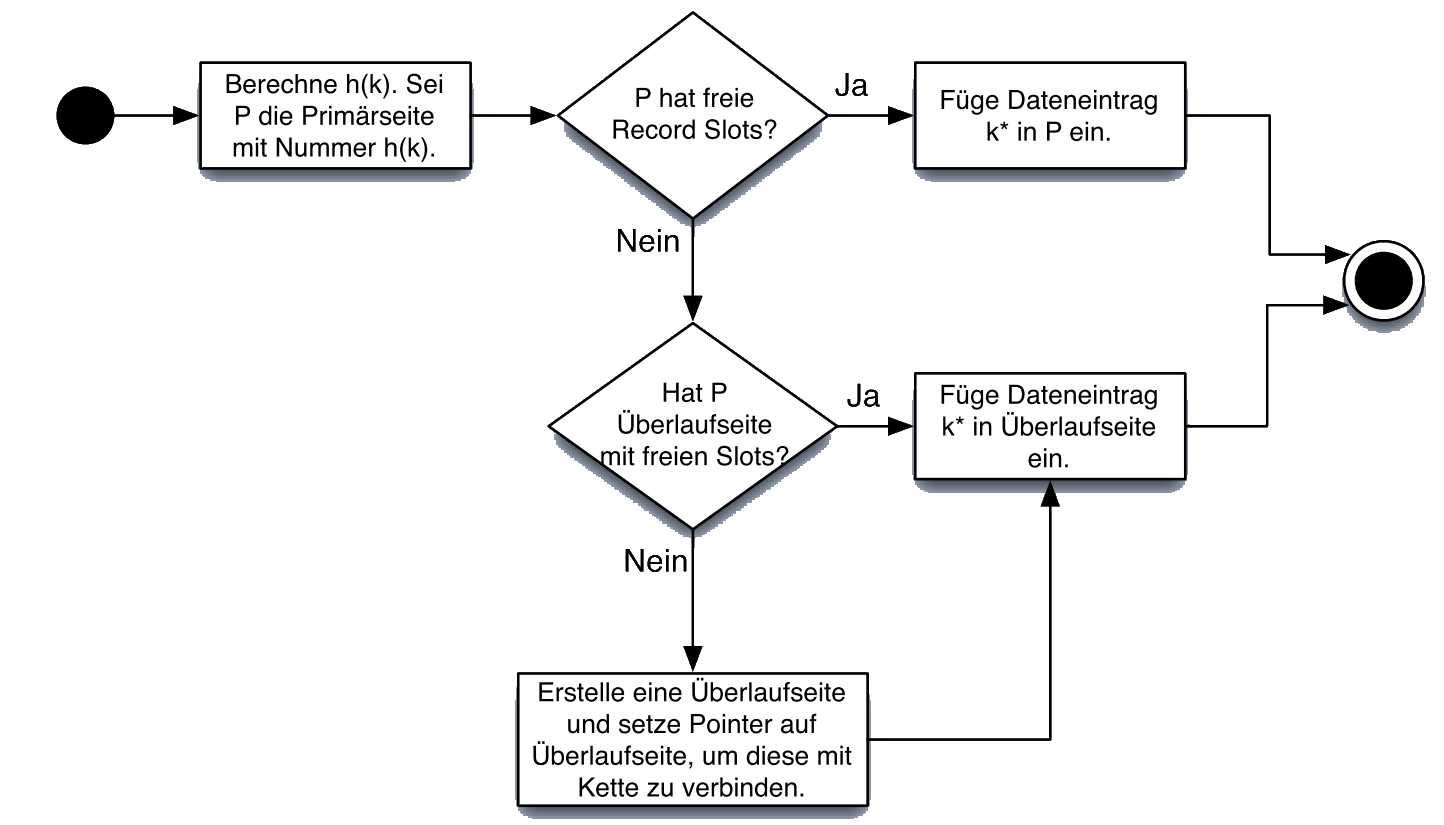
\includegraphics[scale=0.3]{img/Hash-stat-01.png}
\end{figure}
\end{frame}

\begin{frame}{\insertsection}
\framesubtitle{\insertsubsection}	
\structure{L\"oschen eines Datensatzes}
\begin{figure}
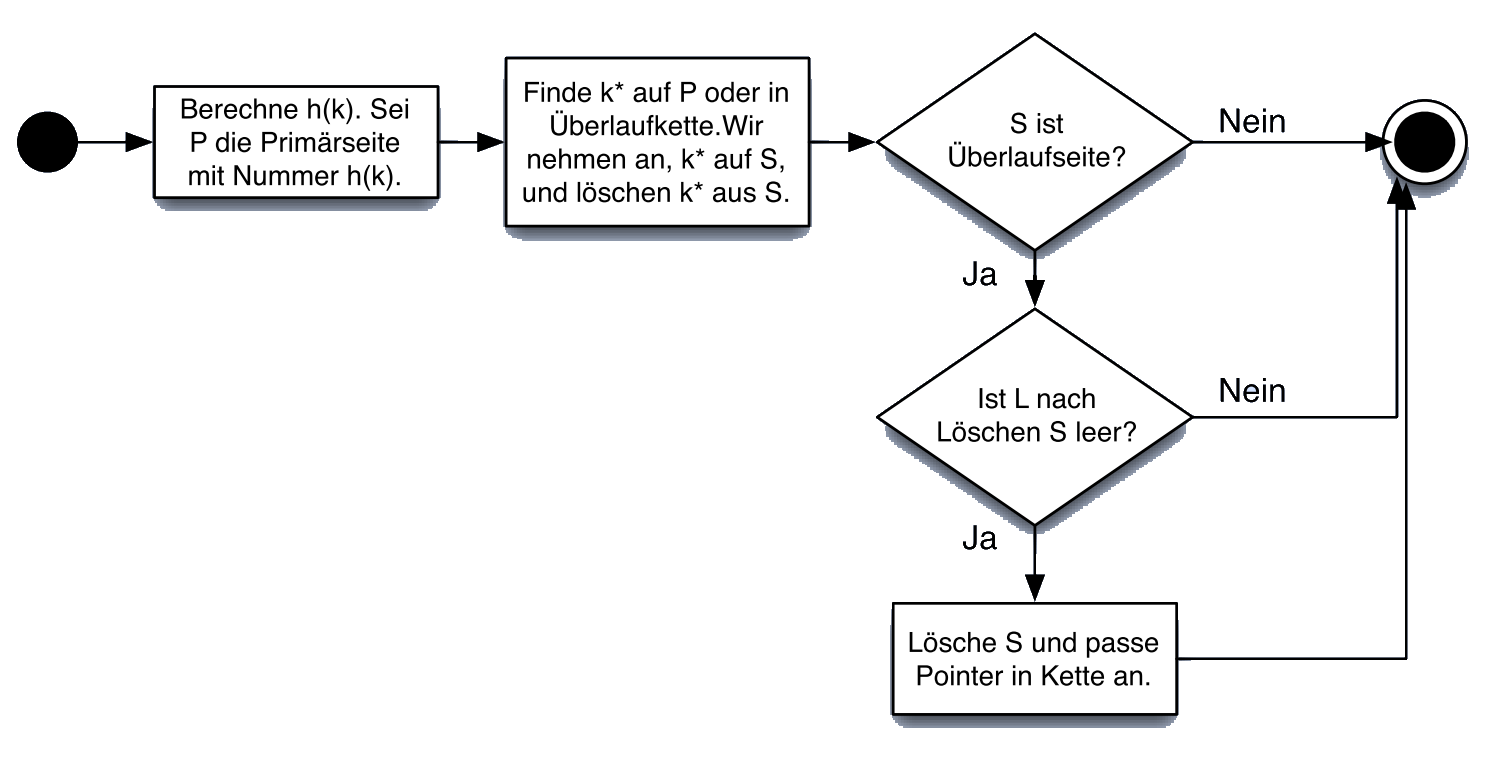
\includegraphics[scale=0.3]{img/Hash-stat-02.png}
\end{figure}
\end{frame}

\begin{frame}{\insertsection}
\framesubtitle{\insertsubsection}	
\structure{Analyse}
\begin{itemize}
\item W\"achst die Datendatei, entstehen \"Uberlaufketten, die I/O-Kosten unvorhersehbar und teurer machen.
\item Schrumpft die Datendatei, kann das zu nahezu leeren Buckets führen.
\item Teure Index-Reorganisation muss durchgef\"uhrt werden.	
\end{itemize}
\end{frame}

\subsection{Erweiterbares Hashing}

\begin{frame}{\insertsection}
\framesubtitle{\insertsubsection}	
\structure{\textbf{Erweiterbares Hashing}}
\abs
\structure{Zielsetzung}
\begin{itemize}
	\item Vermeidung langer \"Uberlaufketten, um Zugriffe auf Hintergrundspeicher gering und voraussehbar zu halten.
\end{itemize}
\abs
\structure{L\"osungsansatz}
\begin{itemize}
	\item Verwendung eines Verzeichnisses, das Index-Hash-Werte auf Pointer von Buckets abbildet.
	\item Seitenüberlauf im Bucket: Neuer Bucket und Verdoppelung des Verzeichnisses -- wenn m\"oglich. 	
\end{itemize}
%\abs
%\textbf{Vorerst: Datens\"atze lassen sich durch Hash-Werte identifizieren.}  
\end{frame}

\begin{frame}{\insertsection}
\framesubtitle{\insertsubsection}	
\structure{Idee}
\begin{itemize}
	\item Hash-Wert $h(s)$ wird f\"ur jeden Index-Wert $s$ ermittelt.
	\item Adressverzeichnis: Weist dem Hash-Wert $h(s)$ die Adresse $P$ des Buckets des Datensatzes mit Feldwert $s$ zu.
	\item Hash-Wert $h(s)$ wird als Bit-Folge betrachtet.
\end{itemize}
\end{frame}

\begin{frame}{\insertsection}
\framesubtitle{\insertsubsection}	
\structure{Idee}
\abs
Adressverzeichnis entspricht balanciertem Bin\"arbaum (genauer: DAG).
	\begin{itemize}
		\item Innere Knoten: $0$-$1$-Abfrage 
		\item Blatt: Pointer auf Bucket
		\item Zwei Kanten je innerem Knoten mit $0$ oder $1$ bezeichnet.
	\end{itemize}
\end{frame}

\begin{frame}{\insertsection}
\framesubtitle{\insertsubsection}	
\structure{\textbf{Formale Beschreibung}}
\begin{columns}[T]
	\begin{column}{.72\textwidth}
		{\small Hash-Funktion: $h: S\to \{0,1\}^n$ ($S$ Dom\"ane der Index-Werte).}
		\begin{itemize}
			\item {\small L\"ange $n$ {gro\ss} genug, um alle Objekte auf Buckets abzubilden.}
		\end{itemize}
		\pause
		{\small Verzeichnis als bin\"arer Entscheidungsbaum}
		\begin{itemize}
			\item {\small Bin\"arer Pfad entlang Hash-Code $h(s)$ f\"ur Index-Wert $s$.}
			\item {\small Traversiere entlang Bit-Folge von $h(s)$ ab f\"uhrendem Bit zum Bucket-Pointer $P$.}
			\item {\small In diesem Bucket liegt ggf.~der Datensatz zum Index-Wert $s$.}
			\pause
			\item {\small Bin\"arer Pfad bis zum Bucket-Pointer $P$ kann bereits durch Pr\"afix $\beta$ von $h(s)=\beta\,\ldots$ 
				eindeutig bestimmt sein.}
			\begin{itemize}
				\item {\small Dann gilt: Alle Pfade der Form $h(\tilde s)=\beta\,\gamma$ f\"uhren zu diesem Pointer $P$.}
				\item {\small L\"ange des minimalen Pr\"afix dieser Art: $\Lambda(P) =$ \emph{lokale Tiefe} von $P$.}
			\end{itemize}
			\pause
			\item {\small \emph{Globale Tiefe} $\Gamma =\max_{\text{$P$ Pointer im Baum}}(\Lambda(P))$}
		\end{itemize}
		%	 \item Bei \"Uberlauf eines Buckets muss weiterer Bucket und ggf.~weitere Entscheidungsstufe eingebaut werden. 
	\end{column}
	\onslide
	\begin{column}{.27\textwidth}
		\begin{figure}
			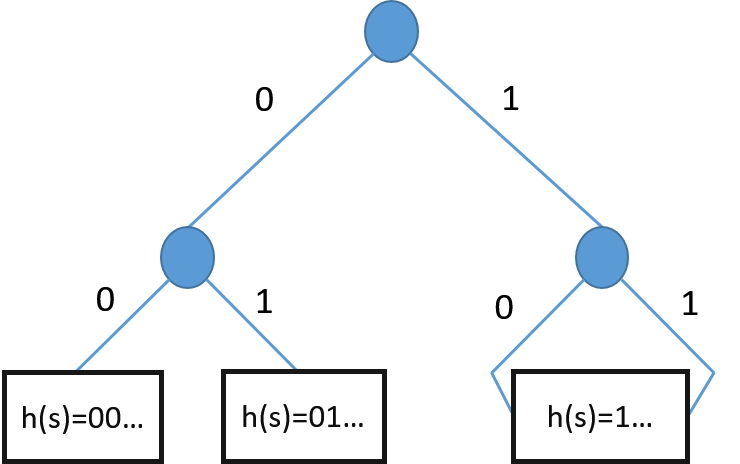
\includegraphics[scale=0.35]{img/Hash-ext-concept-01.png}
		\end{figure}
	\end{column}
\end{columns}
\end{frame}

\begin{frame}{\insertsection}
\framesubtitle{\insertsubsection}	
\structure{Initialisieren, Suchen, Einf\"ugen}
\begin{itemize}
	\item \textbf{Initialisierung}
	\begin{itemize}
		\item Noch kein Index-Wert angelegt.
		\item Lege Pointer auf neues Bucket f\"ur die beiden Bin\"ar-Suchpfade der L\"ange 1 an.
	\end{itemize}
	\pause
	\item \textbf{Suchen}
	\begin{itemize}
		\item Die f\"uhrenden Bits (Pr\"afix) der Bit-Folge $h(s)$ bestimmen Bin\"ar-Suchpfad im Bin\"arbaum zum Bucket, 
		in dem der Datensatz ggf.~liegt.
	\end{itemize}
	\pause
	\item \textbf{Einf\"ugen}
	\begin{itemize}
		\item Suche entsprechenden Bucket. Einf\"ugen des Datensatzes in Bucket.
		\pause
		\item Bei \"Uberlauf des Bucket wird der Baum um weitere Knoten und Kanten erweitert: \texttt{OVERFLOW}
	\end{itemize}	
\end{itemize}
\end{frame}

\begin{frame}{\insertsection}
\framesubtitle{\insertsubsection}	
\structure{Einf\"ugen -- \textbf{\texttt{OVERFLOW}}}
\begin{itemize}
	\item Bucket $B$ (im Pointer $P$) hat maximalen F\"ullstand. Neuer Datensatz kann nicht eingef\"ugt werden.
	\ \\[4pt]
	\item Fallunterscheidung
	\begin{itemize}
		\item Hash-Wert-Pr\"afix der L\"ange $\Lambda(P)+1$ des neuen Datensatzes im Bucket bereits vorhanden
		\begin{itemize}
			\item L\"osung: Verkettete Buckets (bei weiterem Einf\"ugen als ein Bucket betrachtet)
		\end{itemize} 
		\ \\[4pt]
		\item Hash-Wert-Pr\"afix der L\"ange $\Lambda(P)+1$ des neuen Datensatzes im Bucket nicht vorhanden
		\begin{itemize}
			\item Lokale Tiefe kleiner als globale Tiefe: $\Lambda(P)<\Gamma$
			\item Lokale Tiefe gleich globale Tiefe: $\Lambda(P)=\Gamma$
		\end{itemize}
	\end{itemize}
\end{itemize}
\end{frame}

\begin{frame}{\insertsection}
\framesubtitle{\insertsubsection}	
\structure{Einf\"ugen -- \textbf{\texttt{OVERFLOW}}}
\\[4pt]
Lokale Tiefe kleiner globale Tiefe: $\Lambda(P)<\Gamma$
\begin{itemize}
\item Alle Bin\"ar-Suchpfade $h$ zu Bucket-Pointer $P$ splitten erstmals bei Pr\"afix-Pfad der L\"ange $\Lambda(P)$ 
in zwei Teilb\"aume.
\pause
\item Erzeuge neue Buckets $B_0$ und $B_1$ mit Pointer $P_0$ bzw.~$P_1$.
\pause
\item Weise linken Teilbaum dem Pointer $P_0$ und rechten Teilbaum dem Pointer $P_1$ zu.
\pause
\item Verteile die Datens\"atze von $B$ entsprechend ihrer Hash-Codes in $B_0$ und $B_1$.
\pause
\item Setze $\Lambda(B_0)=\Lambda(B_1)=\Lambda(B)+1$
\pause
\item L\"osche Bucket $B$ und Pfad-Pointer-Zuordnung $(h, P)$ im Verzeichnis.
\end{itemize}
\end{frame}

\begin{frame}{\insertsection}
\framesubtitle{\insertsubsection}	
\structure{Einf\"ugen -- \textbf{\texttt{OVERFLOW}}}
\\[4pt]
Lokale Tiefe gleich globale Tiefe: $\Lambda(P)=\Gamma$
\begin{itemize}
\item Nur ein Bin\"ar-Suchpfad $h$ zu Bucket-Pointer $P$.
\pause
\item Erzeuge neue Buckets $B_0$ und $B_1$ mit Pointer $P_0$ bzw.~$P_1$.
\pause
\item Erweitere im Baum den Pfad $h$ zu $h_0=h\circ 0$ und $h_1=h\circ 1$.
\pause
\item Weise $h_0$ dem Pointer $P_0$ und $h_1$ dem Pointer $P_1$ im Verzeichnis/Baum zu.
\pause
\item Verteile die Datens\"atze von $B$ entsprechend ihrer Hash-Codes in $B_0$ und $B_1$.
\pause
\item Setze $\Lambda(B_0)=\Lambda(B_1)=\Lambda(B)+1$ und $\Gamma :=\Gamma + 1$.
\pause
\item L\"osche Bucket $B$ und Pfad-Pointer-Zuordnung $(h,P)$.
\pause
\item F\"ur die Buckets $\tilde B$ mit Pointer $\tilde P \ne P$ im Baum:
\begin{itemize}
\item L\"osche alle Pfad-Pointer-Zuordnungen $(\tilde h, \tilde P)$ im Verzeichnis.
\item Weise $\tilde h\circ 0$ und $\tilde h\circ 1$ dem Pointer $\tilde P$ im Verzeichnis/Baum zu.
\end{itemize}
\end{itemize}	
\end{frame}

\begin{frame}{\insertsection}
\framesubtitle{\insertsubsection}
\structure{\textbf{Demo: Einf\"ugen (schematisch)}}
\onslide<1>\ \ \ \ \ \ \ \ Initialisierung
\begin{figure}\onslide
	\centering	
	\includegraphics<1>{img/Hash-ext-ins-demo-01.png}
	\includegraphics<2>{img/Hash-ext-ins-demo-02.png}
	\includegraphics<3>{img/Hash-ext-ins-demo-03.png}
	\includegraphics<4>{img/Hash-ext-ins-demo-04.png}
	\includegraphics<5>{img/Hash-ext-ins-demo-05.png}
	\includegraphics<6>{img/Hash-ext-ins-demo-06.png}
	\includegraphics<7>{img/Hash-ext-ins-demo-07.png}
	\includegraphics<8>{img/Hash-ext-ins-demo-08.png}
	\includegraphics<9>{img/Hash-ext-ins-demo-09.png}
	\includegraphics<10>{img/Hash-ext-ins-demo-10.png}
	\includegraphics<11>{img/Hash-ext-ins-demo-11.png}
	\includegraphics<12>{img/Hash-ext-ins-demo-12.png}
	\includegraphics<13>{img/Hash-ext-ins-demo-13.png}
\end{figure}
\end{frame}

\begin{frame}{\insertsection}
\framesubtitle{\insertsubsection}	
\structure{\textbf{L\"oschen}}
\\[4pt]
\begin{itemize}
\item L\"oschen des Datensatzes im Bucket.
%\pause
\item Verschmelzung zweier benachbarter Buckets, wenn Dateninhalte in einen Bucket passen.
\begin{itemize}
\item Benachbarte Buckets: Nur letztes Bit des Bin\"ar-Suchpfades verschieden
\end{itemize}		
\item Leere Buckets werden entfernt und Bin\"ar-Suchpfade zusammengef\"uhrt
%\pause
\item Adressverzeichnis wird angepasst 
\begin{itemize}
\item Update von Zuweisung des Bin\"ar-Suchpfads zu Pointer 
\item Halbierung ($\cong$ eine Tiefe weniger im Baum), wenn f\"ur keinen Bucket 
die lokale Tiefe mit der globalen Tiefe \"ubereinstimmt.
\end{itemize}		
\end{itemize}	
\end{frame}

\begin{frame}{\insertsection}
\framesubtitle{\insertsubsection}	
\begin{block}{\textbf{\"Ubungsaufgabe}}
Bauen Sie das Verzeichnis (Bin\"arbaum)	des Hash-Index f\"ur folgende Daten auf:
\abs
Tabelle: \texttt{Mitarbeiterdaten}
\nl
Index f\"ur: \texttt{Mitarbeiter-ID} (\texttt{int})
\nl
Hash-Funktion: gespiegelte binäre \texttt{Mitarbeiter-ID}
\texttt{
\abs  
h(004) = 00100000     (4\ \ = 0..0000100)
\nl
h(007) = 11100000     (7\ \ = 0..0000111)
\nl
h(009) = 10010000     (9\ \ = 0..0001001)
\nl
h(013) = 10110000     (13 = 0..0001101)
\nl
h(019) = 11001000     (19 = 0..0010011)
\nl
h(033) = 10000100     (33 = 0..0100001)
\nl
h(049) = 10001100     (49 = 0..0110001)
\nl
h(051) = 11001100     (51 = 0..0110011)
}
\end{block}
\end{frame}

\nowrite{
%%%%%%%%%%%%%%%%%%%%%%%%%%%%%%%%%%%%%%%%%%%%%%%%%%%%%%%%%%%%%%%%%
\begin{frame}{\insertsection}
	\framesubtitle{\insertsubsection}
	\structure{Beispiele:}
	\begin{itemize}
		\item Kundendatensätze sollen nach Kundennummer sortiert gespeichert werden. 
		\item Die Kundennummern starten bei 0 
	\end{itemize}
	\structure{Lösungsansatz:}
	\begin{itemize}
		\item Speicherung in einem Array \texttt{kunden}, damit ein effizienter Zugriff $O(1)$ gewährleistet ist. 
	\end{itemize}
	\structure{Folge:}
	\begin{itemize}
		\item Kunde 0 in \texttt{kunde[0]} gespeichert, Kunde 1 in \texttt{kunde[1]}, Kunde $i$ in \texttt{kunde[i]}		
	\end{itemize}
	\structure{Erweiterung}
	\begin{itemize}
		\item Für Geschäftskunden werden neue Kundennummern vergeben, die bei 100.000 beginnen
		\item Für Regierungen werden eigene Kundennummern vergeben, die bei 10.000.000 beginnen
	\end{itemize}
	\alert{Das Array beinhaltet ab dem ersten Regierungskunden mindestens 10.000.000 Einträge. Es wird sehr viel Speicherplatz verschwendet.}
\end{frame}
%
\begin{frame}{\insertsection}
	\framesubtitle{\insertsubsection}
	\structure{Eine konkrete Hashfunktion zur Speicherzuweisung}	
	Die Schlüsselmenge kann potentiell unendlich groß werden, während der Speicherplatz begrenzt ist. Eine Hashfunktion kann hier 
	abhilfe schaffen. Gegeben ist die folgende Hashfunktion: 	
	$$h(k) = k \mod m$$ 
	\begin{itemize}
		\item Die Hashfunktion $h$ bestimmt die Position der Eingabe $k$ in einem Array. 
		\item Der Wert von $m$ bestimmt die Größe des Arrays
	\end{itemize}
\end{frame}
%
\begin{frame}{\insertsection}
	\framesubtitle{\insertsubsection}
	\structure{Beispiel: $h(k)= k \mod 5$}
	\begin{itemize}
		\item Kundennummer 1: $h(1) =  1 \mod 5 = 1 \Rightarrow$ \texttt{kunden[1]}
		\item Kundennummer 4: $h(4) =  4 \mod 5 = 4 \Rightarrow$ \texttt{kunden[4]}
		\item Kundennummer 12: $h(12) =  12 \mod 5 = 2 \Rightarrow$ \texttt{kunden[2]}
		\item Kundennummer 10003: $h(10003) =  10003 \mod 5 = 3 \Rightarrow$ \texttt{kunden[3]}
		\item \alert{Kundennummer 3: $h(3) =  3 \mod 5 = 3 \Rightarrow$ \texttt{kunden[3]}}		
	\end{itemize}	
	\alert{Da die möglichen Eingabewerte $k$ zahlreicher sind als die verfügbaren Speicherzellen, ist es meist nicht vermeidbar, dass es zu Hashkollisionen kommt.}	
\end{frame}
%
\begin{frame}{\insertsection}
	\framesubtitle{\insertsubsection}
	\structure{Hashkollisionen:}	
	\alert{Da die Menge der Schlüsselwerte mächtiger ist als die Menge der verfügbaren Speicherplätze, sind Hashkollisionen wahrscheinlich. Seine $s_1,s_2 \in S, s_1 \neq s_2$ und $w\in W$. Eine Hashkollision liegt vor, falls gilt:}	
	$$h(s_1) = w = h(s_2)$$	
	Eine Hashkollision im Sinne der Datenbanktechnik bedeutet, dass ein Speicherplatz für einen Datensatz bereits belegt ist. Hashkollisionen können durch einige Verfahren aufgelöst werden: 
	\begin{itemize}
		\item Lineares Sondieren
		\item Anhängen einer verketteten Liste an die Hash-Position (Overflow-Listen)
		\item Mehrfaches Hashing, d.h. Anwendung weiterer Hash-Funktionen 
	\end{itemize}	
\end{frame}
%
\begin{frame}{\insertsection}
	\framesubtitle{\insertsubsection}
	\structure{Lineares Sondieren}	
		Wird eine Kollision festgestellt, so wird der nächste freie Speicherplatz ausgehend von der berechneten Hashposition gesucht.		
	\structure{Beispiel: $h(k)= k \mod 5$,  $k=\{1,2,1003,3\}$}	
	\vspace{5mm}
	\begin{center}
		\begin{tabular}{|c|c|c|c|c|c|}\hline
			Index $h(k)$ & 0 & 1 & 2 & 3 & 4  \\\hline\hline
			Wert & &1&2 & 1003 &\cellcolor{Yellow}3 \\\hline
		\end{tabular}
	\end{center}	
	Der Wert $3$ wird an Position $4$ gespeichert, da das Feld $3$ bereits von der 1003 belegt ist. 
\end{frame}
%
\begin{frame}{\insertsection}
	\framesubtitle{\insertsubsection}
	\structure{Lineares Sondieren}	
	\begin{itemize}
		\item Schnelle Berechnung des nächsten Speicherplatzes 
		\item Bei häufigen Hashkollisionen leidet die Performance und degeneriert zur Laufzeit einer verketteten Liste
		\item Speicherplatz kann nicht dynamisch erweitert werden: Irgend wann ist das Array voll.
	\end{itemize}	
\end{frame}
%
\begin{frame}{\insertsection}
	\framesubtitle{\insertsubsection}
	\structure{Verkettete Listen}
	\begin{itemize}
		\item Wird eine Kollision festgestellt, so wird an der Array-Position eine verkettete Liste angehangen, die die Werte speichert
		\item Die berechnete Position bleibt erhalten
	\end{itemize}
	\structure{Beispiel: $h(k)= k \mod 5$, $k=\{1,2,1003,3\}$}	
	\vspace{5mm}
	\begin{center}
		\begin{tabular}{|c|c|c|c|p{7mm}|c|}\hline
			Index $h(k)$ & 0 & 1 & 2 & 3 & 4  \\\hline\hline
			Wert & &1&2 & \cellcolor{Yellow}1003\newline 3 & \\\hline
		\end{tabular}
	\end{center}
\end{frame}
%
\begin{frame}{\insertsection}
	\framesubtitle{\insertsubsection}
	\structure{Verkettete Listen}	
	\begin{itemize}
		\item Hashkollisionen erzeugen verkettete Listen
		\item Bei häufigen Hashkollisionen leidet auch hier die Performance und degeneriert zur Laufzeit einer verketteten Liste
		\item Speicherplatz kann dynamisch vergeben werden
	\end{itemize}	
	\structure{Generelles zu Hashfunktionen}	
	\begin{itemize}
		\item Hashkollisionen sind quasi unvermeidbar
		\item Tradeoff zwischen: 
		\begin{itemize}
			\item Speicherbedarf
			\item Geschwindigkeit / Laufzeitverhalten
		\end{itemize}
		\item Die meisten Hashfunktionen können mittels Parametern konfiguriert werden (z.B. die Wahl eines geeigneten $m$ bestimmt die Menge des verwendeten Speicherplatzes und hat Auswirkungen auf die Anzahl der Hashkollisionen
	\end{itemize}	
\end{frame}
%
\begin{frame}{\insertsection}
	\framesubtitle{\insertsubsection}	
	\structure{Eine Hash-Funktion muss nicht unbedingt eine Zahl als Eingabe bekommen:}
	\begin{itemize}
		\item Werden Hashfunktionen mit Strings gebildet, so muss eine Verrechnung stattfinden
		\begin{itemize}
			\item Die Hashfunktion $h$ könnte z.B. zuerst den ASCII-Code der jeweiligen Zeichen addieren 
			\item Beispiel: \texttt{A=65, B=66, C=67} 
			\item $h(\mathtt{'ABC'}) = 198$
		\end{itemize}
		\item In objektorientierten Programmiersprachen werden die Objekte oft mittels eines Hashwertes identifiziert 
		\item Auch ganze Dateien können mit Hashwerten belegt werde, z.B. für die Berechnung von Checksummen
		\begin{itemize}
			\item Beispiel: 128Bit md5-Hash einer Datei \texttt{test.txt}: \texttt{a3cca2b2aa1e3b5b3b5aad99a8529224}
		\end{itemize}
	\end{itemize}
\end{frame}
%
\begin{frame}{\insertsection}
	\framesubtitle{\insertsubsection}
	\structure{Statisches Hashing im Datenbank-Kontext}
	\begin{itemize}
		\item Konsekutive (d.h. direkt hintereinander auf Festplatte befindliche) Blöcke werden in \textit{Buckets} zusammengefasst (Alternativ: Ein Bucket = ein Block)
		\item In jedem Bucket befinden sich mehrere Records
		\item Hashfunktion berechnet für einen Schlüssel die passende Bucketnummer 
		\item Hashtabelle bildet Bucketnummer auf eine Blockadresse ab
		\item Hashtabelle wird im Dateiheader mitgeführt, da sie sehr klein ist.
	\end{itemize}	
	\alert{Die genaue Kentniss der Hash-Funktion ist in diesem Kontext nicht notwendig}	
\end{frame}
%
\begin{frame}{\insertsection}
\framesubtitle{\insertsubsection}	
\begin{figure}
\includegraphics[scale=0.7]{img/statischesHashing.png}
\caption{Statisches Hashing mit Hashtabelle und Datenbuckets (Quelle: \cite[S. 610]{EN10})}
\end{figure}	
\end{frame}
%
\begin{frame}{\insertsection}
	\framesubtitle{\insertsubsection}
	\structure{Was passiert, wenn ein Bucket voll ist?}
	\begin{itemize}
		\item Anhängen von verketteten Listen möglich
		\item Am Ende eines Buckets werden Record Pointer gespeichert
		\begin{itemize}
			\item Zeiger auf ein relatives Bucket
			\item Zeiger auf den Datensatz innerhalb des Buckets
		\end{itemize}
		\item In den Overflow-Listen können wiederum Record Pointer auf weitere Records existieren. Auf diese Weise können mehrfache Hashkollisionen abgefangen werden
	\end{itemize}	
	\alert{Gefahr bei zahlreichen Hashkollisionen: Aufwand strebt in Richtung des Aufwands einer verketteten Liste.}
\end{frame}
%
\begin{frame}{\insertsection}
	\framesubtitle{\insertsubsection}	
	\begin{center}
		\begin{figure}
			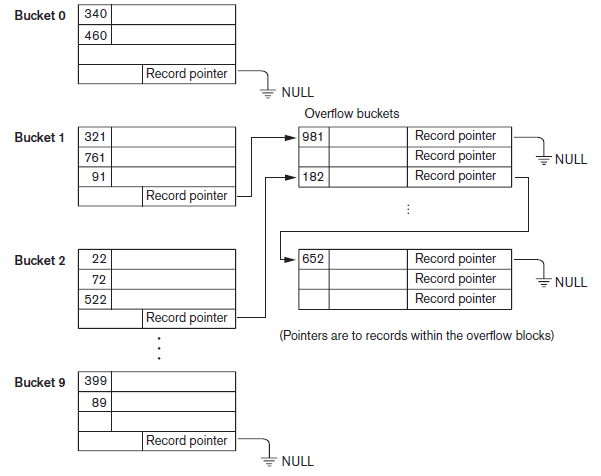
\includegraphics[width=200pt]{img/buckets.png}
			\caption{Hashverfahren mit Overflow-Buckets (Quelle: \cite[S. 611]{EN10})}
		\end{figure}
	\end{center}	
\end{frame}
%
\begin{frame}{\insertsection}
	\framesubtitle{\insertsubsection}
	\structure{Statisches Hashing}
	\begin{itemize}
		\item Kann nur für eine statische Anzahl von $M$ Buckets verwendet werden
		\item Falls nur wenig Datensätze in der Hashtabelle sind, wird viel Speicherplatz 
		verschwendet, da die statische Hashtabelle immer für $M$ Buckets vollständig aufgebaut wird
		\item Bei zu vielen Datensätzen (und daraus resultierenden Hashkollisionen) wird die Performance schlechter und nähert sich der Performance einer verketteten Liste an.
	\end{itemize}
	\alert{Achtung: Wir befinden uns immer noch auf der Ebene einer Datei! Es ist daher sehr aufwändig, eine statische Hashdatei ad hoc zu vergrößern oder zu verkleinern!}	
	$\Rightarrow$ Erweiterbares Hashing	
\end{frame}
%
\begin{frame}{\insertsection}
	\framesubtitle{\insertsubsection}
	\structure{Eigenschaften des erweiterbaren Hashings:}
	\begin{itemize}
		\item Es wird eine dynamische Hashtabelle verwaltet, die je nach Bedarf wachsen oder schrumpfen kann
		\item Dem entsprechend existiert auch eine dynamische Anzahl an Buckets, die nach Bedarf allokiert oder gelöscht werden können
		\item Die Hashfunktion berechnet für einen gegebenen Eingabeschlüssel eine Bit-Sequenz
		\begin{itemize}
			\item $h(\mathtt{'Meier'}) = 0 0 1 0 1$
			\item $h(\mathtt{'Mueller'}) = 0 0 1 1 0$
		\end{itemize}	
	\end{itemize}	
\end{frame}
%
\begin{frame}{\insertsection}
	\framesubtitle{\insertsubsection}
	\structure{Das erweiterbare Hashing ist ein Nachfolger des statischen Hashings}
	\begin{itemize}
		\item Es wird ein globales Verzeichnis von Bucket-Adressen geführt 
		\item Die globale Tiefe des Verzeichnis wird $d$ genannt 
		\item Das globale Verzeichnis speichert $2^d$ Einträge (Bucket-Adressen) 
		\item Die ersten $d$ Bits eines Hash-Wertes bestimmen das Target Bucket 
		\item Es existieren maximal $2^d$ Buckets, die Buckets können aber auch zusammengefasst werden: 
		\begin{itemize}
			\item $d'$ wird lokale Tiefe genannt 
			\item Die lokale Tiefe bestimmt die Anzahl der höherwertigen Bits, die den Inhalt des Buckets ausmachen
		\end{itemize}
	\end{itemize}		
\end{frame}
%
\begin{frame}{\insertsection}
	\framesubtitle{\insertsubsection}
	\begin{center}
		\begin{figure}
				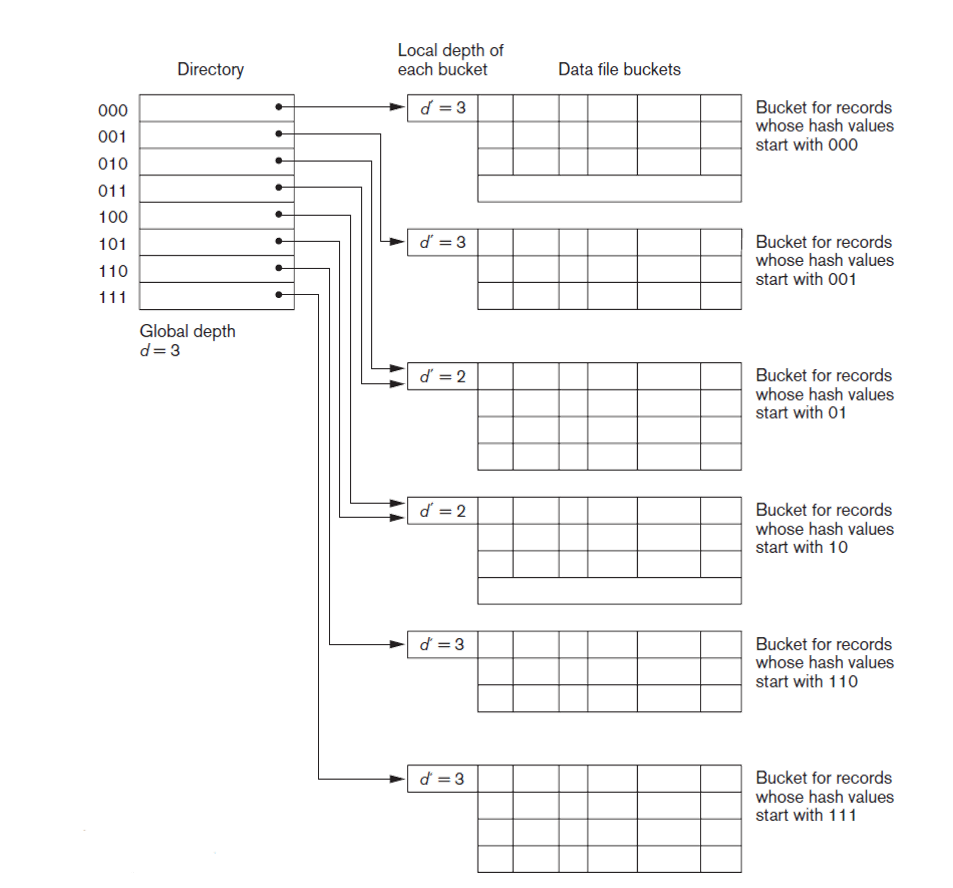
\includegraphics[width=180pt]{img/extHash.png}
			\caption{Erweiterbares Hashing (Quelle: \cite[S. 613]{EN10})}
		\end{figure}
	\end{center}
\end{frame}
%
\begin{frame}{\insertsection}
	\framesubtitle{\insertsubsection}
	\structure{Vorgehen:}
	\begin{itemize}
		\item Start: $d=0$
		\begin{itemize}
			\item Es existiert ein globales Verzeichnis mit genau einem Eintrag auf ein Bucket
			\item In das Bucket werden alle Records geschrieben (da die ersten $d=0$ Bits verwendet werden)
		\end{itemize}
	\end{itemize}		
	\begin{center}
		\begin{figure}
			\begin{tikzpicture}[list/.style={rectangle split, rectangle split parts=2,
				draw, rectangle split horizontal}, >=stealth, start chain]			
			\node[list, on chain] (d0) {0}; 
			\node (d) [above=1mm of d0] {$d=0$}; 
			\node (dstrich) [right=3cm of d] {$d'=0$}; 
			\node[draw, rectangle] (b00) [below=0mm of dstrich, minimum width=2cm] {\textit{Leer}}; 
			\node[draw, rectangle] (b01) [below=0cm of b00, minimum width=2cm] {\textit{Leer}}; 			
			\draw[*->] let \p1 = (d0.two), \p2 = (d0.center) in (\x1,\y2) -- (b00); 			
			\end{tikzpicture}
		\end{figure}
	\end{center}
	\alert{Alle Records werden in das existierende Bucket geschrieben, bis ein Überlauf erreicht wird.}
\end{frame}
%
\begin{frame}{\insertsection}
	\framesubtitle{\insertsubsection}
	\structure{Überlauf-Regelung}
	\begin{itemize}
		\item Ist ein Bucket voll, so wird anhand der folgenden Regel verfahren: 
		\begin{itemize}
			\item falls $d' < d$, so splitte das Bucket und erhöhe $d'$ um den Wert $1$ (sowohl für das alte als auch das neue Bucket)
			\item falls $d' = d$, so wird $d$ und $d'$ um den Wert $1$ inkrementiert. Damit verdoppelt sich die Größe des globalen Verzeichnisses. Auch hier müssen die Buckets gesplittet werden 
		\end{itemize}
	\end{itemize}	
	\vspace{6mm}
	\begin{columns}
		\begin{column}{.48\textwidth}
			\begin{center}
				\begin{figure}
					\begin{tikzpicture}[list/.style={rectangle split, rectangle split parts=2,
						draw, rectangle split horizontal}, >=stealth, start chain]										
					\node[list, on chain] (d0) {0}; 
					\node (d) [above=1mm of d0] {$d=0$}; 					
					\node (dstrich) [right=2cm of d] {$d'=0$}; 
					\node[draw, rectangle] (b00) [below=0mm of dstrich, minimum width=2cm] {\textit{Meier}}; 
					\node[draw, rectangle] (b01) [below=0cm of b00, minimum width=2cm] {\textit{Müller}}; 					
					\draw[*->] let \p1 = (d0.two), \p2 = (d0.center) in (\x1,\y2) -- (b00); 
					\end{tikzpicture}	
				\end{figure}				
			\end{center}
		\end{column}		
		\begin{column}{.48\textwidth}
			\structure{Hash-Werte:}			
			\begin{tabular}{|c|c|}\hline
				\textbf{\small Schlüssel} & \textbf{\small Hashwert}\\\hline
				\texttt{\small Meier} & \small 001\\\hline
				\texttt{\small Mueller} & \small 101\\\hline
				\texttt{\small Schulz} & \small 110 \\\hline
			\end{tabular}
		\end{column}		
	\end{columns}	
	\vspace{1mm}	
	\alert{Alle Records werden in das existierende Bucket geschrieben, bis ein Überlauf erreicht wird.}
\end{frame}
%
\begin{frame}{\insertsection}
	\framesubtitle{\insertsubsection}
	\structure{Überlauf-Regelung}
	\begin{itemize}
		\item In diesem Fall gilt: $d'=d$, d.h. $d$ und $d'$ wird um 1 inkrementiert und das Bucket wird gesplittet
		\item Die Records werden anhand der führenden $d$ Bits des Hashwertes aufgeteilt.
	\end{itemize}
	\vspace{6mm}
	\begin{columns}
		\begin{column}{.48\textwidth}
			\begin{center}
				\begin{figure}
					\begin{figure}
						\begin{tikzpicture}[list/.style={rectangle split, rectangle split parts=2,
							draw, rectangle split horizontal}, >=stealth, start chain]												
						\node[list, on chain] (d0) {0}; 
						\node[list, on chain] (d1) [below=0mm of d0] {1}; 
						\node (d) [above=1mm of d0] {$d=1$}; 						
						\node (dstrich) [right=2cm of d] {$d'=1$}; 
						\node[draw, rectangle] (b00) [below=0mm of dstrich, minimum width=2cm] {\textit{Meier}}; 
						\node[draw, rectangle] (b01) [below=0cm of b00, minimum width=2cm] {\textit{Leer}}; 						
						\node (dstrich2) [below=2mm of b01] {$d'=1$}; 						
						\node[draw, rectangle] (b10) [below= 1mm of dstrich2, minimum width=2cm] {\textit{Müller}}; 
						\node[draw, rectangle] (b11) [below= 0mm of b10, minimum width=2cm] {\textit{Schulz}}; 						
						\draw[*->] let \p1 = (d0.two), \p2 = (d0.center) in (\x1,\y2) -- (b00); 
						\draw[*->] let \p1 = (d1.two), \p2 = (d1.center) in (\x1,\y2) -- (b10); 
						\end{tikzpicture}	
					\end{figure}
				\end{figure}
			\end{center}
		\end{column}		
		\begin{column}{.48\textwidth}
			\structure{Hash-Werte:}			
			\begin{tabular}{|c|c|}\hline
				\textbf{\small Schlüssel} & \textbf{\small Hashwert}\\\hline
				\texttt{\small Meier} & \small 001\\\hline
				\texttt{\small Mueller} & \small 101\\\hline
				\texttt{\small Schulz} & \small 110 \\\hline
			\end{tabular}
		\end{column}		
	\end{columns}	
\end{frame}
%
\begin{frame}{\insertsection}
	\framesubtitle{\insertsubsection}
	\structure{Dynamisches Hashing verhindert keine Hash-Kollisionen!}
	\begin{itemize}
		\item Auch hier kommt das Konzept einer Overflow-Liste zum Einsatz. 
	\end{itemize}	
	\begin{columns}
		\begin{column}{.48\textwidth}
			\begin{center}
				\begin{figure}
					\begin{tikzpicture}[list/.style={rectangle split, rectangle split parts=2,
						draw, rectangle split horizontal}, >=stealth, start chain]										
					\node[list, on chain] (d0) {0}; 
					\node[list, on chain] (d1) [below=0mm of d0] {1}; 
					\node (d) [above=1mm of d0] {$d=1$}; 					
					\node (dstrich) [right=2cm of d] {$d'=1$}; 
					\node[draw, rectangle] (b00) [below=0mm of dstrich, minimum width=2cm] {\textit{Meier}}; 
					\node[draw, rectangle] (b01) [below=0cm of b00, minimum width=2cm] {\textit{Leer}}; 					
					\node (dstrich2) [below=2mm of b01] {$d'=1$}; 					
					\node[draw, rectangle] (b10) [below= 1mm of dstrich2, minimum width=2cm] {\textit{Müller}}; 
					\node[draw, rectangle] (b11) [below= 0mm of b10, minimum width=2cm] {\textit{Schulz}}; 					
					\node[draw, rectangle] (o) [below right=2mm of b11, minimum width=2cm] {Schroeder}; 					
					\draw[*->] let \p1 = (d0.two), \p2 = (d0.center) in (\x1,\y2) -- (b00); 
					\draw[*->] let \p1 = (d1.two), \p2 = (d1.center) in (\x1,\y2) -- (b10);
					\draw[*->] (b11.south) -- (o.west); 
					\end{tikzpicture}	
				\end{figure}
			\end{center}
		\end{column}		
		\begin{column}{.48\textwidth}
			\structure{Hash-Werte:}			
			\begin{tabular}{|c|c|}\hline
				\textbf{\small Schlüssel} & \textbf{\small Hashwert}\\\hline
				\texttt{\small Meier} & \small 001\\\hline
				\texttt{\small Mueller} & \small 101\\\hline
				\texttt{\small Schulz} &\cellcolor{Yellow} \small 110 \\\hline
				\texttt{\small Schroeder} &\cellcolor{Yellow} \small 110 \\\hline
			\end{tabular}
		\end{column}		
	\end{columns}	
\end{frame}
%%%%%%%%%%%%%%%%%%%%%%%%%%%%%%%%%%%%%%%%%%%%%%%%%%%%%%%%%%%%%%%%%
}

\section{Anwendungen von Indizes}

\begin{frame}[fragile]{\insertsection}
\framesubtitle{\insertsubsection}
\structure{Indexerstellung in SQL:}	
\lstset{language=sql}
\lstset{captionpos=b}		
\begin{lstlisting}[numbers=none, xleftmargin=3ex]
CREATE [UNIQUE] INDEX nameIdx ON person(nachname)
\end{lstlisting}		
\begin{itemize}
	\item Erzeugt Index auf Attribut \texttt{nachname} der Relation \texttt{person}
	\item Schlüsselwort \texttt{UNIQUE} gibt an, ob Index eindeutig sein soll. Das hei\ss t, Index-Feld enth\"alt 
	keine doppelten Werte.
	\item Fast alle RDBMS erzeugen dabei einen Index in Form eines $B^+$-Baumes. 
	\item Erstellen eines Index sollte in Erwägung gezogen werden, wenn Attributmenge in folgenden Abfragen häufig vorkommt: 
	\begin{itemize}
		\item \texttt{WHERE}, \texttt{GROUP BY}, \texttt{DISTINCT}, \texttt{ORDER BY }
	\end{itemize}
	\item Erstellen eines Index sollte in Erwägung gezogen werden, wenn Lesezugriffe im Vergleich zu L\"osch- und Einf\"ugezugriffen
	\"uberwiegen.
	\item Auf einer Relation können mehrere Indexstrukturen erstellt werden, diese müssen dann aber auch vom RDBMS gepflegt werden.
\end{itemize}	
\end{frame}

\begin{frame}{\insertsection}
\framesubtitle{\insertsubsection}
\structure{Hash-Indizes können eingesetzt werden, wenn:}
\begin{itemize}
\item Feld, auf dem die Hash-Funktion arbeitet, Schlüsseleigenschaften besitzt (Minimierung von Kollisionen)
\item Lesezugriffe deutlich \"uberwiegen
\item Exact-Match-Suchanfragen gestellt werden (\texttt{ ... WHERE id = 4711}))
\end{itemize}
Hashdateien sollten nicht eingesetzt werden bei:
\begin{itemize}
\item vielen gleichen Attributwerten auf dem Suchfeld (z.~B.~Attribut \texttt{plz} in einer Kundentabelle 
-- Overflow-Listen entstehen)
\item Bereichsabfragen (z.B. \texttt{... WHERE knr $>$ 5000})
\end{itemize}
\end{frame}

\begin{frame}[fragile]{\insertsection}
\framesubtitle{\insertsubsection}
\structure{Man kann das RDBMS aber auch dazu auffordern, mit einem Hash-Index zu arbeiten:}
\lstset{language=sql}
\lstset{captionpos=b}
\begin{lstlisting}[xleftmargin=3ex, numbers=none, caption=Relation mit gehashtem Primärschlüssel (MS SQL Server)]
CREATE TABLE Person (
pid INT NOT NULL, 
Vorname nvarchar(20) NOT NULL,
Nachname nvarchar(20) NOT NULL,
PRIMARY KEY NONCLUSTERED HASH (pid) WITH (BUCKET_COUNT = 100)
);
\end{lstlisting}
Der Code erzeugt 
\begin{itemize}
\item Relation mit Namen \texttt{Person}
\item Drei Attribute \texttt{pid, Vorname, Nachname}
\item Primärschlüssel auf dem Attribut \texttt{pid} mit Hash-Index
\end{itemize}
\texttt{Achtung: Syntax ist spezifisch für den MS SQL-Server.}
\end{frame}

\begin{frame}[fragile]{\insertsection}
\framesubtitle{\insertsubsection}
\structure{Auch MySQL beherrscht Hash-Indizes:}
\lstset{language=sql}
\lstset{captionpos=b}
\begin{lstlisting}[xleftmargin=3ex, numbers=none, caption=Relation mit gehashtem Primärschlüssel (MySQL)]
CREATE TABLE Person (
pid INT, INDEX USING HASH (pid),
Vorname nvarchar(20) NOT NULL,
Nachname nvarchar(20) NOT NULL
) ENGINE = MEMORY ; 
\end{lstlisting}
MySQL unterstützt gehashte Indizes nur für In-Memory-Tabellen.
\nl
Das Tabellenschema wird auf Festplatte gespeichert; die Tabelle ist also nach Server-Start wieder vorhanden. 
\nl
Die Daten werden aber ausschließlich im Hauptspeicher gehalten.
\end{frame}

\section*{Übungsaufgaben}

\begin{frame}[t]
\frametitle{\insertsection}
\begin{alertblock}{B-B\"aume}
\begin{enumerate}
\item Erstellen Sie einen B-Baum der Ordnung $k=3$ für das Wort \texttt{LUDWIGSHAFEN}
\item Löschen Sie die Buchstaben \texttt{W, A} und \texttt{L} aus dem B-Baum der vorigen Aufgabe
\item Erstellen Sie einen B-Baum der Ordnung $k=5$ und fügen Sie die Zahlen von $1\dots20$ in sortierter Reihenfolge in den Baum ein.
Welche Beobachtung können Sie machen und welche Schlüsse ziehen Sie daraus?
\end{enumerate}
\end{alertblock}
\end{frame}

\begin{frame}[t]
\frametitle{\insertsection}
\begin{alertblock}{Indexing und Hashing}
\begin{enumerate}
\item Erläutern Sie den Begriff einer Hash-Kollision und begründen Sie, warum sich Hash-Kollisionen praktisch nicht vermeiden lassen.
\item Gegeben sei die Hash-Funktion $h(k)=k \mod 10$.
\begin{enumerate}
\item \label{a} Erstellen Sie eine Hashtabelle und fügen Sie die Zahlen 1,2,4,6,8,12 ein. Welches Problem ergibt sich?
\item Lösen Sie das Problem aus Aufgabenteil \ref{a} durch die Verwendung einer Overflow-Liste und fügen Sie zusätzlich die Werte 12, 13, 15, 42, 1337 ein.
%\item Lösen Sie das Problem aus Aufgabenteil \ref{a} durch lineares Sondieren und fügen Sie zusätzlich die Werte 12, 13, 15, 42, 1337 ein.
\end{enumerate}
\item Begründen Sie, welche Eigenschaften ein Attribut aufweisen muss, damit eine Hash-Struktur sinnvoll  bzw. nicht  sinnvoll ist. 
\end{enumerate}
\end{alertblock}
\end{frame}

\begin{frame}[t]
\frametitle{\insertsection}
\begin{alertblock}{Indexing und Hashing}
Gegeben ist die folgende Relation sowie die folgende Hash-Wert-Tabelle:
\abs
{\scriptsize{
\begin{tabular}{|l|l|l|l|l|}\hline
\multicolumn{4
}{|c|}{\textbf{Personen}}\\\hline
\textbf{KNR} &\textbf{Nachname} & \textbf{Vorname}  & \textbf{Ort} \\\hline\hline
4710 &Mustermann &Max  &Siegen \\
4711 &Musterfrau &Erika  &Wilnsdorf \\
4712 &Schwarzer &Manfred  &Mannheim \\
4713 &Hefeker &Christian  &Siegen \\
4714 &Otter &Timo &Mannheim \\
4715 &Hetzelbach &Frank  &Wilnsdorf \\
4716 &Schmidt &Karl  &Nürnberg \\
4717 &Hetzel &Ottmar  &Mosbach \\
4718 &Schmidt & Hubert  &Mannheim \\
4719 &Voigtländer &Harry  &Fulda \\
4720 &Petersen &Piet &Norderney \\\hline
\end{tabular}
\hfill
\begin{tabular}{|l|l|}\hline
\textbf{Ort} & $h(\mathsf{Ort})$ \\\hline\hline
Siegen & 0010 1101 1111 1011 0010 1100 0011 0000\\
Wilnsdorf & 1111 0001 0010 0100 1001 0011 0110 1101\\
Mannheim & 0100 0011 1010 1100 1100 0110 1101 1111\\
Norderney & 1010 0011 1010 0000 1100 0110 1001 1111\\
Nürnberg & 1100 0111 1110 1101 1011 1111 0011 1010\\
Fulda & 0011 0101 1010 0110 1100 1001 1110 1011\\
Mosbach & 1001 1000 0011 1111 1001 1100 0000 0001\\\hline
\end{tabular}
}}
\abs
Organisieren Sie die Daten mit einem Hash-Index mittels erweiterbarem Hashing. 
\nl
Gehen Sie davon aus, dass ein Bucket lediglich Platz für zwei Personen-Records bietet.
\end{alertblock}
\end{frame}
